% ===================================================================
% CONSOLIDATED THESIS - single self-contained file (all text + citations).
% Auto-assembled from the modular sources. Compile: lualatex -> biber -> lualatex x2.
% ===================================================================
\documentclass{scrbook}


%% Setting document options:

%%% Layout settings
	\KOMAoptions{
		fontsize=12pt,
		bibliography=totoc,
		headings=normal,
		toc=listof,
		toc=indent,
		listof=indent,
		listof=totoc,
		twoside=false
	}
	\setcounter{tocdepth}{2} % show subsections in TOC (useful for methodology chapter)
	\usepackage{geometry, setspace}
	\geometry{
		paper=a4paper,
		hmargin=30mm,
		top=15mm,
		bottom=20mm,
		includeheadfoot,
	}
	\onehalfspacing
	% Move chapter headings up slightly:
	\renewcommand*{\chapterheadstartvskip}{\vspace*{-1.48\topskip}}


%% Setting the font:
	\usepackage{lmodern}


%% Setting up headers and footers:
	\usepackage[headsepline=false]{scrlayer-scrpage}
	\automark[chapter]{chapter}
	\lohead{}
	\cohead{\headmark}
	\rohead{}
	\lofoot{}
	\cofoot*{\pagemark}
	\rofoot{}
	\pagestyle{scrheadings}


%% Language selection:
	\usepackage{polyglossia}
	\setmainlanguage{english}
	\setotherlanguage{german}


%% Settings for tables
	\usepackage{tabularray}
	\UseTblrLibrary{amsmath, booktabs, siunitx}


%% Settings for citations and bibliography:
	\usepackage{csquotes}
	\usepackage[
		backend=biber,
		style=authoryear, 
		uniquename=init, 
		giveninits=true, 
		maxbibnames=3, 
		minbibnames=2
	]{biblatex} 
	\addbibresource{references.bib}
	\defbibheading{head}{\chapter{References}}
	% Colon after last author
	\renewcommand*{\labelnamepunct}{\addcolon\addspace}
	% All names as last name, first name
	\DeclareNameAlias{sortname}{family-given}
	% Ensure that citations with multiple authors have a "," in the text and in the bibliography
	\renewcommand*{\finalnamedelim}{\addspace\bibstring{and}\addspace}
	% --- Make the ENTIRE citation (author + year) one clickable link, not just the year ---
	\usepackage{ifthen}
	\makeatletter
	\DeclareFieldFormat{citehyperref}{%
	  \DeclareFieldAlias{bibhyperref}{noformat}% avoid nested links
	  \bibhyperref{#1}}
	\renewbibmacro*{cite}{%
	  \printtext[citehyperref]{%
	    \iffieldundef{shorthand}
	      {\ifthenelse{\ifnameundef{labelname}\OR\ifentrytype{jurisdiction}}
	         {\usebibmacro{cite:label}}
	         {\printnames{labelname}}%
	       \setunit{\printdelim{nameyeardelim}}%
	       \usebibmacro{cite:labelyear+extrayear}}
	      {\usebibmacro{cite:shorthand}}}}
	\renewbibmacro*{textcite}{%
	  \printtext[citehyperref]{%
	    \ifnameundef{labelname}
	      {\usebibmacro{cite:label}}
	      {\printnames{labelname}}%
	    \setunit{\printdelim{nametitledelim}}%
	    \usebibmacro{cite:labelyear+extrayear}}}
	\makeatother


%% Other packages:
	\usepackage{
		float,      % Placement of floats
		graphicx,   % Inclusion of graphics
		hologo,     % TeX logos
		mathtools,  % Math typesetting (loads amsmath)
		microtype,  % Microtypographic improvements
		paralist,   % Space-saving lists
		xcolor,     % Color support
	}

%% Additional packages for econometrics thesis:
	\usepackage{amssymb}        % Additional math symbols
	\usepackage{bm}             % Bold math symbols (e.g., vectors/matrices)
	\usepackage{dcolumn}        % Decimal-aligned columns in tables
	\usepackage{threeparttable} % Tables with notes (for regression output)
	\usepackage{subcaption}     % Subfigures (e.g., side-by-side IRF plots)
	\usepackage{enumitem}       % Better list control


%% LaTeX searches for images in the specified locations:
	\graphicspath{{./images/},{./},{../../Output/figures/}}


%% Automatic PDF links in the document:
	\usepackage[
		colorlinks=true,
		linkcolor=black,
		citecolor=blue,
		urlcolor=black,
		pdfborder={0 0 0},
	]{hyperref}


%% Custom math commands for the thesis:
	% Abnormal return
	\newcommand{\AR}{\mathrm{AR}}
	% Cumulative abnormal return
	\newcommand{\CAR}{\mathrm{CAR}}
	% Expected value
	\newcommand{\E}{\mathbb{E}}
	% Variance
	\newcommand{\Var}{\mathrm{Var}}
	% Covariance
	\newcommand{\Cov}{\mathrm{Cov}}
	% Correlation
	\newcommand{\Corr}{\mathrm{Corr}}
	% DCC correlation
\begin{document}
\frontmatter

\begin{titlepage}

\begin{center}

\vspace*{1.2cm}

\huge {\bfseries
The Dollar's Safe-Haven Status Across Two Shocks: Evidence from Liberation Day and the Strait of Hormuz Crisis}\\[1cm]

\Large {Bachelor's Thesis}\\[1cm]

\large {Department of Economics}\\[0.2cm]

\large {University of Mannheim}\\[0.5cm]

\end{center}

\vfill

\noindent submitted to:\\
Dr.\ Husnu C.\ Dalgic\\[1cm]
submitted by:\\
Leon Weigele\\[1cm]
Matriculation Number: 1957464\\
Degree Program: Bachelor of Science in Economics (B.Sc.)\\[1cm]
Address: Stamitzstraße 5, 68167 Mannheim\\
Phone Number: +49 1756208327\\
Email: leon.weigele@students.uni-mannheim.de\\[1cm]
Mannheim, \today

\setcounter{page}{0}

\end{titlepage}
\tableofcontents


%% Abbreviations List
\chapter*{List of Abbreviations}\label{av}
\addcontentsline{toc}{chapter}{List of Abbreviations}
\markboth{List of Abbreviations}{List of Abbreviations}
\begin{tabular}{ll}
ADF   & Augmented Dickey--Fuller \\
CAR   & Cumulative Abnormal Return \\
CIP   & Covered Interest Parity \\
DCC   & Dynamic Conditional Correlation \\
DXY   & U.S.\ Dollar Index \\
EM    & Emerging Market \\
EPU   & Economic Policy Uncertainty \\
FEVD  & Forecast Error Variance Decomposition \\
GARCH & Generalized Autoregressive Conditional Heteroskedasticity \\
GPR   & Geopolitical Risk \\
IRF   & Impulse Response Function \\
SVAR  & Structural Vector Autoregression \\
TPU   & Trade Policy Uncertainty \\
VIX   & CBOE Volatility Index \\
\end{tabular}

%% List of Figures
\listoffigures

%% List of Tables
\listoftables

%% Symbol List
\chapter*{List of Symbols}\label{sv}
\addcontentsline{toc}{chapter}{List of Symbols}
\markboth{List of Symbols}{List of Symbols}
\begin{tabular}{ll}
$R_{i,t}$          & Return of asset $i$ at time $t$ \\
$\AR_{i,t}$        & Abnormal return of asset $i$ at time $t$ \\
$\CAR_{i}(t_1,t_2)$ & Cumulative abnormal return over window $[t_1, t_2]$ \\
$h_{i,t}$          & Conditional variance of asset $i$ at time $t$ \\
$\rho_{ij,t}$      & Time-varying conditional correlation between $i$ and $j$ \\
$\alpha, \beta$     & GARCH parameters \\
$\alpha_{\text{DCC}}, \beta_{\text{DCC}}$ & DCC parameters \\
$D_k$              & Crisis dummy variable for event $k$ \\
$\varepsilon_t$    & Structural shock vector \\
\end{tabular}
\mainmatter

% ---------- 01_introduction ----------

\chapter{Introduction}
\label{ch:introduction}

Within a single year, two major shocks moved global markets in opposite directions for the
U.S.\ dollar. On 2~April 2025---``Liberation Day''---the United States announced sweeping
tariffs on virtually all of its trading partners, and the dollar \emph{fell}: it depreciated
against the euro, the yen and the Swiss franc even as equities sold off and volatility
spiked, the textbook conditions under which the dollar normally \emph{rises}. Less than a
year later, as escalation in the Gulf threatened to close the Strait of Hormuz and sent
crude sharply higher, the dollar did exactly what the safe-haven literature predicts---it
appreciated. Two episodes, both with the United States implicated, produced a mirror image.
This thesis asks why.

The puzzle speaks to a live debate about whether the dollar's exceptional status is eroding.
A growing literature argues that the currency's safe-haven premium has weakened, pointing to
the unusual co-movement of a falling dollar, rising Treasury yields and rising risk premia
during the 2025 tariff episode \parencite{corsetti2025,kamin2025,obstfeld2023,jiang2026}.
Against this, the long tradition on the dollar's ``exorbitant privilege'' and its role as the
world's reserve and safe-haven currency \parencite{gourinchasrey2005,habib2012,ranaldo2010}
implies the status should be durable. The two 2025--2026 shocks offer an unusually clean
natural experiment for adjudicating the debate, because they differ in \emph{kind}: one is a
U.S.\ trade-policy shock, the other a geopolitical oil-supply shock.

\section*{Research question}

The central question of this thesis is therefore: \emph{does the dollar's safe-haven
response depend on the type of shock---even when the United States is, in some sense, the
originator of both?} The design contrasts three episodes. The Liberation Day tariff
announcement is a purely U.S.-originated economic-policy shock. The 2026 Israel--Iran/Hormuz
crisis is a geopolitical oil-supply shock in which the United States is implicated as a
co-belligerent but still functions as a financial safe harbour. And the 2022 Russian
invasion of Ukraine---an external military/oil shock not authored by the United
States---serves as a control for the ``classical'' safe-haven response. Comparing the three
isolates whether the dollar's behaviour is conditioned by the nature of the shock or merely
by who caused it.

\section*{Approach and contribution}

The thesis answers the question with two complementary empirical layers on a single daily
dataset spanning January~2019 to June~2026. An \emph{event study} measures the cumulative
abnormal response of the dollar, a cross-section of currency baskets, gold, equities and
crude oil around each shock, and tests formally whether the dollar's response differs across
events. A \emph{structural vector autoregression} then asks whether geopolitical-risk, oil
and risk-sentiment innovations transmit to the dollar dynamically over the full sample. The
two layers reinforce one another: the event study shows that discrete, dated shocks move the
dollar in opposite directions depending on type, while the VAR shows that the continuous
geopolitical-risk index does not move it at all on an average day, locating the safe-haven
response in identifiable events rather than in ambient geopolitical noise.

The contribution is threefold. First, to the best of the author's knowledge this is the
first systematic side-by-side comparison of the Liberation Day and Iran/Hormuz episodes for
currency markets. Second, the thesis bridges the safe-haven and commodity-currency
literatures by carrying the oil channel and a gold benchmark through the same design,
showing that gold behaves as a hedge \emph{against} the dollar rather than as an
unconditional substitute for it. Third, the rebuilt carry/dollar risk factors and the WMR
currency panel extend standard cross-sectional tools through to mid-2026, allowing the most
recent shocks to be studied with consistent, citable data.

The remainder of the thesis is organised as follows. Chapter~\ref{ch:literature} reviews the
safe-haven, dollar-erosion and commodity-currency literatures and states the predictions
that follow from them. Chapter~\ref{ch:background} narrates the 2025--2026 events.
Chapter~\ref{ch:methodology} describes the data and the event-study and VAR methodologies.
Chapter~\ref{ch:event_study} presents the event-study results, Chapter~\ref{ch:svar} the
structural VAR. Chapter~\ref{ch:discussion} discusses the findings and their implications,
and Chapter~\ref{ch:conclusion} concludes.

% ---------- 02_literature_review ----------

\chapter{Literature Review}
\label{ch:literature}

This chapter situates the thesis within five strands of research---currency
factor models, safe-haven currencies and gold, geopolitical risk, tariff shocks,
and commodity currencies---and closes by distilling them into testable
hypotheses. The unifying question is when, and through which channel, the U.S.\
dollar functions as a safe haven, and whether that function survives when the
United States is itself the source of the shock.


\section{Currency Returns and Factor Models}
\label{sec:lit_currency_factors}

The modern cross-section of currency returns is organised around a small number
of risk factors. \textcite{lustig2011} identify a ``slope'' factor (the return on
a portfolio long high-interest-rate and short low-interest-rate currencies) that
explains most of the cross-sectional variation in carry returns and is tied to
innovations in global equity-market volatility; high-interest-rate currencies
load more heavily on this common factor, so investors in the carry trade are
compensated for bearing global risk. This logic motivates sorting currencies into
portfolios by their exposure to common shocks, and the dollar and carry factors
derived from it underpin the portfolio construction used in
Chapter~\ref{ch:methodology}. Related work on dominant-currency pricing links the
pricing of trade and the currency composition of invoicing to these risk premia
\parencite{dalgic2024,dalgic2025}.

The dollar occupies a special position in this system. \textcite{gourinchasrey2005}
document the United States' ``exorbitant privilege''---a persistent excess return
on its external assets over its liabilities---and \textcite{gourinchas2017} show
that this privilege is mirrored by an ``exorbitant duty'': the hegemon transfers
wealth to the rest of the world precisely during global crises, with transfers of
roughly $19\%$ of U.S.\ GDP during the 2007--2009 financial crisis. \textcite{gourinchas2019}
embed this in a broader account of the international monetary system and a renewed
Triffin dilemma, while \textcite{obstfeld2023} describe a ``global dollar cycle''
in which dollar appreciation tightens financial conditions worldwide. Together these
contributions frame the dollar's safe-haven status as a structural feature of the
international monetary system---and therefore something whose erosion would be
economically consequential.


\section{Safe-Haven Currencies and Gold}
\label{sec:lit_safe_haven}

Following \textcite{baur2010}, an asset is a \emph{hedge} if it is uncorrelated
with risky assets on average and a \emph{safe haven} if it is uncorrelated with
(or negatively correlated with) them specifically during market stress; they find
gold to be a hedge against equities on average and a safe haven in extreme
declines, though the safe-haven property is short-lived. This conditional, crisis-
contingent definition is the one adopted throughout the thesis. Applied to
currencies, \textcite{ranaldo2010} show that the Swiss franc and Japanese yen
appreciate against the dollar when U.S.\ equities fall and volatility rises, with
the effect strengthening non-linearly in the volatility factor and during crises.
\textcite{debock2015} document the same recurrent pattern across risk-off
episodes---the yen, franc and dollar all appreciate against other currencies---and
relate it to fundamentals such as the nominal interest rate and the net foreign
asset position. \textcite{habib2012} push beyond the carry trade to ask what
\emph{makes} a currency a safe haven, finding that the net foreign asset position,
low external vulnerability, and economic size are robustly associated with
safe-haven status, whereas the interest-rate spread against the United States is
not. Methodologically, the time-varying correlation approach used to test these
properties---and applied to gold and other assets by \textcite{kumar2025}---rests
on the dynamic conditional correlation model discussed in Section~\ref{sec:lit_gpr}
and Chapter~\ref{ch:methodology}.


\section{Geopolitical Risk and Currency Markets}
\label{sec:lit_gpr}

\textcite{caldara2022} construct the news-based Geopolitical Risk (GPR) index used
in this thesis, showing that it spikes around wars and major adverse events and
that higher geopolitical risk foreshadows lower investment and employment and
larger downside risks; importantly, they distinguish the \emph{threat} of adverse
events from their \emph{realisation}, a distinction directly relevant to staged
crises such as the Hormuz episode. Building on such measures, \textcite{liu2024}
study geopolitical-risk-sorted currency portfolios and report a positive risk
premium for exposure to geopolitical shocks, and the \textcite{imf2025gfsr} finds
that geopolitical-risk shocks predict currency depreciation and equity declines,
particularly in more vulnerable economies. This literature motivates treating
geopolitical events as priced risk rather than noise, and supplies the GPR series
used as an external control in the empirical chapters.


\section{Tariff Shocks and Exchange Rates}
\label{sec:lit_tariffs}

The 2025 tariff episode has generated a fast-growing literature that is central to
this thesis. \textcite{kamin2025} provides econometric evidence that, following
the Liberation Day announcements of April~2025, the dollar switched from behaving
as a safe haven---appreciating in periods of market volatility---to behaving as a
``risk-on'' currency that moves inversely with volatility. \textcite{jiang2026}
document the same break in historical correlations (the dollar depreciating while
U.S.\ rates rose relative to the euro, the VIX increased, and the dollar
convenience yield fell) and interpret it through shifts in global demand for
dollar safe assets, calibrating a steady-state real dollar depreciation of around
$7.6\%$ should the United States lose reserve-currency demand. \textcite{hassan2025}
provide the theoretical counterpart: in a general-equilibrium model where currency
safety is endogenous, a trade war that isolates U.S.\ goods markets erodes the
dollar's safety premium and raises U.S.\ interest rates. On the empirical
exchange-rate response, \textcite{corsetti2025} construct a tariff-shock database
and show that exchange rates react to U.S.\ tariff shocks systematically once the
size and relevance of the measures (and expected retaliation) are accounted for,
while \textcite{kalemliozcan2026} emphasise the role of tariff \emph{uncertainty}
in the dollar's behaviour. The theoretical tariff--exchange-rate offset is
formalised by \textcite{itskhoki2025}. Policy institutions corroborate the market
dislocation: the \textcite{ecb2025fsr} and the \textcite{ecb2026bulletin} document
trade fragmentation, the pass-through of higher U.S.\ tariffs, and the effects of
trade-policy uncertainty on activity. This thesis contributes a direct event-study
comparison of this trade-policy shock against contemporaneous military/oil-supply
shocks.


\section{Commodity Currencies and Oil}
\label{sec:lit_commodities}

\textcite{chen2003} establish that the U.S.-dollar price of commodity exports
exerts a strong and stable influence on the real exchange rates of commodity
exporters such as Australia, Canada and New Zealand, providing the basis for the
oil-exporter versus oil-importer portfolio split used in
Chapter~\ref{ch:methodology}. The nature of the oil shock matters, however:
\textcite{kilian2009} shows that oil-price movements driven by supply
disruptions, aggregate demand, and precautionary (oil-specific) demand have
distinct macroeconomic consequences, so a price increase caused by a supply scare
is not equivalent to one caused by strong demand---nor to a tariff-induced demand
collapse. This typology maps directly onto the thesis's contrast between the
demand-side tariff shock (falling oil) and the supply-side Hormuz shock (surging
oil). For the 2026 episode specifically, \textcite{fattouh2026} provide a detailed
anatomy of the Strait of Hormuz oil shock and the associated disruption to Gulf
output, while \textcite{kilian2026} quantify the inflationary consequences of the
2026 Iran war through oil prices, and the \textcite{imf2026menap} documents the
regional and global spillovers, including Brent rising above \$100 per barrel and
the role of the ceasefire in de-escalation.


\section{Hypotheses}
\label{sec:hypotheses}

Taken together, these strands point to a single organising prediction: the dollar's
safe-haven response is conditional on the \emph{type} of shock rather than on whether the
United States is its originator. Both the external benchmark (the 2022 Russian invasion of
Ukraine) and the U.S.-originated Hormuz crisis are military/oil-supply shocks, around which
the safe-haven literature (Section~\ref{sec:lit_safe_haven}) implies the dollar should
appreciate; the Liberation Day tariff announcement, by contrast, is a U.S.\ trade-policy
shock that the dollar-erosion literature (Section~\ref{sec:lit_tariffs}) suggests should
weaken the very currency it originates from. Gold offers a natural counterpoint: as an asset
external to any sovereign it might be expected to bid in \emph{both} kinds of episode, so
that comparing it against the dollar isolates what is specific to the dollar's status
\parencite{baur2010}---a prediction this thesis puts directly to the data. The cross-section
of currencies should in turn sort on the oil channel, exporter currencies outperforming
importers when the Hormuz supply shock lifts crude but losing ground when the tariff shock
depresses oil through weaker demand \parencite{chen2003,kilian2009}.

\noindent The remainder of the thesis puts these predictions to the data: the dollar
and the oil cross-section in the event study of Chapter~\ref{ch:event_study}, with gold
examined alongside them, while the structural VAR of Chapter~\ref{ch:svar} traces the dynamic
responses to orthogonalised geopolitical-risk, oil, and uncertainty shocks.

% ---------- 03_background ----------

\chapter{Background: The Events of 2022--2026}
\label{ch:background}

This chapter narrates the episodes the empirical chapters analyse and fixes the dates used
throughout. Three are central---the 2025 U.S.\ tariff shock, the 2026 Iran/Hormuz crisis,
and the 2022 Russian invasion of Ukraine as an external control---together with two
within-crisis sub-events (the April~2025 tariff pause and the June~2026 ceasefire) that
serve as natural reversals.

\section{Liberation Day and the U.S.\ Tariff Shock}
\label{sec:bg_tariff}

On 2~April 2025, branded ``Liberation Day,'' the United States announced broad tariffs on
nearly all trading partners. The market reaction was severe and, for the dollar,
anomalous. Equities fell sharply, implied volatility spiked, and crude oil dropped as
markets priced weaker global demand---yet the dollar \emph{depreciated} rather than
attracting the usual flight-to-safety bid, sliding several percent against the euro, yen and
Swiss franc. Long-term Treasury yields, after an initial decline, backed up even as the
currency weakened, a co-movement widely read as evidence that the episode dented the
dollar's safe-haven premium rather than reinforcing it \parencite{corsetti2025,ecb2025fsr}.
A partial ninety-day tariff pause on 9~April 2025 tempered the equity drawdown but did not
restore the dollar, suggesting markets treated the shock as a regime change in U.S.\
trade policy rather than a transient surprise.

\section{The Israel--Iran Escalation and the Strait of Hormuz}
\label{sec:bg_iran}

The Gulf episode unfolded in stages. A first, twelve-day confrontation in June~2025
(Israeli and U.S.\ strikes on Iranian facilities, an Iranian response, and a rapid
ceasefire) lifted crude only briefly and left currencies little changed. Escalation resumed
in February~2026 and turned acute on 4~March 2026, when Iran moved to close the Strait of
Hormuz---the conduit for roughly a fifth of seaborne oil---triggering attacks on shipping
and a sharp spike in Brent \parencite{fattouh2026,kilian2026}. The dollar strengthened on
impact, the classical safe-haven response and the mirror image of the tariff episode. A
further round of U.S.\ strikes followed on 28~May 2026, and a sixty-day ceasefire announced
on 11~June 2026, committing to reopen the Strait, reversed much of the move in both crude and
the dollar---providing a clean within-crisis test of whether the premium that the threat put
into the dollar came back out on de-escalation.

\section{The Ukraine Control}
\label{sec:bg_ukraine}

The Russian invasion of Ukraine on 24~February 2022 is the external benchmark: a
military/oil-supply shock not authored by the United States. It produced the textbook
pattern---a sustained dollar appreciation alongside a jump in energy prices---and so anchors
what a ``classical'' safe-haven response looks like when the United States is a bystander
rather than a protagonist.

\section{Event Timeline}
\label{sec:bg_timeline}

\begin{table}[htbp]
\centering
\begin{threeparttable}
\caption{Event timeline and shock classification}
\label{tab:timeline}
\small
\begin{tabular}{l l l l}
\toprule
Date & Event & Type & Oil \\
\midrule
2022-02-24 & Russia invades Ukraine        & External military/oil (control) & $\uparrow$ \\
2025-04-02 & Liberation Day tariffs         & U.S.\ trade policy             & $\downarrow$ \\
\quad 2025-04-09 & \quad 90-day tariff pause & \quad sub-event                & $\downarrow$ \\
2025-06-13 & Twelve-day war (Israel/U.S.--Iran) & U.S.-implicated military   & $\uparrow$ (mild) \\
2026-02-28 & Hormuz crisis begins           & U.S.-implicated oil supply     & $\uparrow\uparrow$ \\
\quad 2026-03-04 & \quad Strait of Hormuz closed & \quad sub-event            & $\uparrow\uparrow$ \\
2026-05-28 & U.S.\ strikes on Iran          & U.S.-implicated military       & $\uparrow$ \\
2026-06-11 & Sixty-day ceasefire            & de-escalation                  & $\downarrow$ \\
\bottomrule
\end{tabular}
\begin{tablenotes}[flushleft]\footnotesize
\item \textit{Notes.} ``Type'' classifies each shock by origin and nature; the final column
gives the qualitative crude-oil response. Sub-events are reversals nested within their
parent episode.
\end{tablenotes}
\end{threeparttable}
\end{table}

\section{Key Variables Over the Sample}
\label{sec:bg_descriptive}

Figure~\ref{fig:overview} plots the broad dollar index, the VIX, crude oil and the
geopolitical-risk index over 2019--2026, with the four headline events shaded. The visual
record previews the central result: the dollar rises into the Ukraine and Hormuz bands but
falls through the Liberation Day band, while oil and risk gauges move with the geopolitical
episodes. The formal analysis follows in Chapters~\ref{ch:event_study}
and~\ref{ch:svar}.

\begin{figure}[htbp]
  \centering
  
\includegraphics[width=\linewidth]{fig1_overview}
  \caption[Key variables, 2019--2026]{Key variables over the sample with the four main events
  shaded (Ukraine invasion, Liberation Day, twelve-day war, Hormuz crisis). Sources: FRED,
  LSEG, and Caldara and Iacoviello's Geopolitical Risk index \parencite{caldara2022}.}
  \label{fig:overview}
\end{figure}

% ---------- 04_data_methodology ----------

\chapter{Data and Methodology}
\label{ch:methodology}

% Target: 5-6 pages


\section{Data}
\label{sec:data}

\subsection{Exchange Rates and Financial Variables}
\label{sec:data_fx}

The currency panel comprises 32 exchange rates against the U.S.\ dollar, sampled daily from
1~January 2019 to 30~June 2026. Spot rates are taken from LSEG/Refinitiv at the WM/Reuters
(WMR) fixing and exported as a single consistent panel; the Federal Reserve's H.10 release
(via FRED) serves as a cross-check. All rates are expressed as foreign currency per U.S.\
dollar, so that a rise denotes dollar appreciation; the four rates LSEG quotes in the opposite
convention (EUR, GBP, AUD, NZD) are inverted accordingly. Daily returns are log changes,
$r_{i,t}=\ln(S_{i,t-1}/S_{i,t})$, signed so that a positive value is an appreciation of the
foreign currency against the dollar.

The macro-financial block is drawn from FRED: the broad, advanced-economy and
emerging-market nominal dollar indices (\texttt{DTWEXBGS}, \texttt{DTWEXAFEGS},
\texttt{DTWEXEMEGS}); the 5- and 10-year Treasury yields (\texttt{DGS5}, \texttt{DGS10}), the
5-year TIPS yield (\texttt{DFII5}) and 5-year breakeven inflation (\texttt{T5YIE}); the VIX
(\texttt{VIXCLS}); Brent and WTI crude (\texttt{DCOILBRENTEU}, \texttt{DCOILWTICO}); Henry Hub
natural gas (\texttt{DHHNGSP}); and the S\&P~500 (\texttt{SP500}). Three series not carried by
FRED are taken from LSEG: the gold spot price (\texttt{XAU=ZKBZ}, USD/oz), the Euro Stoxx~50
price index (\texttt{.STOXX50E}, EUR) and the Dutch TTF front-month natural-gas contract
(\texttt{TRNLTTFMc1}, EUR/MWh). Indices, equities and commodities enter as log returns;
yields and the VIX enter in first differences.

\subsection{Geopolitical and Policy Uncertainty Indices}
\label{sec:data_gpr}

Geopolitical risk is measured by the Caldara and Iacoviello (2022) Geopolitical Risk (GPR)
index, used at daily frequency---with its \emph{threat} and \emph{act} sub-indices---and
monthly, downloaded from the authors' site. Policy uncertainty is captured by the U.S.\ daily
Economic Policy Uncertainty (EPU) index and the Trade Policy Uncertainty (TPU) index from
\textit{policyuncertainty.com}. The dollar and carry risk factors are reconstructed from spot
and one-month forward exchange rates following Lustig, Roussanov and Verdelhan (2011): the
one-month forward discount $f_{i,t}-s_{i,t}$ proxies the interest-rate differential under
covered interest parity; currencies are sorted on this signal each month, and the dollar
factor (the average forward-implied excess return) and the carry factor (the high-minus-low
portfolio return) are formed. Rebuilding the factors from current market data extends them
through the 2026 sample, replacing the course-supplied series that end in 2017.

\subsection{Portfolio Construction}
\label{sec:data_portfolios}

Two basket schemes are used. The first sorts currencies by their average one-month forward
discount over the sample into terciles: the low-yield tercile forms the \emph{safe} (funding)
basket and the high-yield tercile the \emph{risky} (carry) basket, with pegged and managed
currencies (DKK, HKD, SAR, KWD, CNY) excluded from the sort. This is the classification that
underlies the carry factor and the main event-study specification. Because the low-yield
tercile also contains low-rate Asian currencies that are not conventional safe havens, a
second, literature-standard scheme is reported as a robustness check: a \emph{named-haven}
safe basket of the yen, Swiss franc and euro against a \emph{risky} basket of the Turkish
lira, Brazilian real, South African rand, Mexican peso, Colombian peso and Indonesian rupiah.
Independently, currencies are split by net oil-trade position into oil exporters (NOK, CAD,
MXN, COP, BRL, SAR, KWD) and oil importers (JPY, KRW, INR, THB, TWD, TRY). All baskets are
equally weighted; the equal-weighted average of all currency returns defines the dollar
basket (\texttt{USD\_EW}).


\section{Event Study Methodology}
\label{sec:method_event}

The main specification is the \emph{constant-mean return} model. For each series $i$ the
normal return is its average over an estimation window of $[-130,-11]$ trading days
preceding the event; the abnormal return on day $t$ of the event window is the deviation
from that mean,
\begin{equation}
  \AR_{i,t} = R_{i,t} - \hat\mu_i, \qquad
  \hat\mu_i = \frac{1}{120}\sum_{s=-130}^{-11} R_{i,s},
\end{equation}
and the cumulative abnormal return aggregates these over the window,
\begin{equation}
  \CAR_i(t_1,t_2) = \sum_{t=t_1}^{t_2} \AR_{i,t}.
\end{equation}
The event window is $[-20,+20]$ trading days. Cumulative windows $\CAR(0,h)$ for
$h\in\{1,5,10,20\}$ capture the announcement reaction, while a long horizon $\CAR(0,50)$
---estimated on $[-170,-51]$ so the estimation window does not overlap the wider event
window---gauges persistence. The significance of a single CAR is assessed with
$t=\CAR/(\hat\sigma_i\sqrt{L})$, where $\hat\sigma_i$ is the estimation-window standard
deviation of $\AR_i$ and $L=t_2-t_1+1$. The difference between two events' CARs is tested
with $\Delta=\CAR_A-\CAR_B$ and standard error
$\sqrt{L\,(\hat\sigma_A^2+\hat\sigma_B^2)}$, treating the (non-overlapping) event windows
as independent.

The constant-mean model is preferred to the market model because the object of study is
the dollar itself. The natural market factor for the currency baskets is the dollar
factor, which is endogenous to the response under examination: regressing dollar exchange
rates on a dollar factor would absorb the common dollar movement into $\beta_i R_{m,t}$
and leave little in the abnormal return. As a robustness check on \emph{individual}
currencies, the market model
\begin{equation}
  R_{i,t} = \alpha_i + \beta_i R_{m,t} + \varepsilon_{i,t}, \qquad
  \AR_{i,t} = R_{i,t} - (\hat\alpha_i + \hat\beta_i R_{m,t}),
\end{equation}
with $R_{m,t}$ the equal-weighted dollar factor, is reported in
Appendix~\ref{ch:appendix_a} and leaves the safe-haven hierarchy unchanged. Where
cross-sectional dependence across currencies is a concern, the Kolari and Pynnönen (2010)
adjusted test can replace the plain $t$-test; given the small number of non-overlapping
events, that refinement is relegated to the appendix.


% DCC-GARCH dropped — thesis scoped to the event study (Ch.~5) and the structural VAR (Ch.~6).


\section{Structural VAR}
\label{sec:method_svar}

% TODO: 7-variable daily VAR (2020--2026):
% GPR, Brent, VIX, EPU/TPU, Safe basket, Risky basket, DXY
% TODO: Cholesky ordering — GPR most exogenous, currencies most endogenous
% TODO: Lag selection: AIC/BIC via VAR.select_order()
% TODO: Stationarity checks (ADF), stability (eigenvalues inside unit circle)
% TODO: Impulse response functions (1-20 days), bootstrapped confidence bands
% TODO: Subsample comparison: tariff period vs. Iran period
% TODO: Optional: FEVD

% ---------- 05_event_study ----------
%
% Chapter 5 — Event Study Results.
% Numbers generated by Code/03_event_study.py, 04_event_study_w50.py,
% 05_cross_event_tests.py (constant-mean model); verified against
% Data/processed/event_study/*.csv. Tables are \input from their own files.
% Figures resolve via \graphicspath (settings.tex now includes ../../Output/figures/).

\chapter{Event Study Results}
\label{ch:event_study}

This chapter measures how the U.S.\ dollar, the cross-section of currency baskets, and
crude oil responded to four shocks. The design isolates the thesis's central contrast:
three of the shocks are \emph{U.S.-originated} (the Liberation Day tariff announcement,
the twelve-day war, and the 2026 Hormuz crisis), while the 2022 Russian invasion of
Ukraine is an \emph{external} military/oil shock in which the United States is not the
instigator, and which therefore serves as a benchmark for the ``classical'' safe-haven
response. Abnormal returns are computed with a constant-mean model: the normal return of
each series is its mean over the estimation window $[-130,-11]$ trading days, the
abnormal return is the deviation from that mean, and the cumulative abnormal return
$\CAR(0,h)$ sums abnormal returns from the event day through trading day~$h$.%
\footnote{The constant-mean specification is preferred to the market model here because
the object of study is the dollar itself: the natural ``market'' factor for the currency
baskets is the dollar factor, which is endogenous to the response we seek to measure and
would absorb the common dollar movement into $\beta\,R_{m,t}$. The market model with the
dollar factor is therefore reported only as a robustness check on \emph{individual}
currencies (Appendix~\ref{ch:appendix_a}). See Section~\ref{sec:method_event}.}
Significance is assessed with a $t$-test on the CAR, $t=\CAR/(\hat\sigma_{\text{est}}
\sqrt{L})$. Tables~\ref{tab:es_dollar_horizon} and~\ref{tab:es_cross_section} collect the
headline numbers; the discussion below reads them event by event.

% Event-study results tables. % !TEX root = ../mainfile.tex
% Event-study results tables. % !TEX root = ../mainfile.tex
% Event-study results tables. % !TEX root = ../mainfile.tex
% Event-study results tables. \input{content/tab_event_study_results} where needed,
% or copy the two table environments individually.
% Numbers generated by Code/03_event_study.py and Code/04_event_study_w50.py
% (constant-mean model, estimation window [-140,-21]; [-170,-51] for h=50).
% Verified against Data/processed/event_study/*.csv (re-run 2026-07-20).

\begin{table}[htbp]
\centering
\begin{threeparttable}
\caption{The U.S.\ dollar's response by event and horizon}
\label{tab:es_dollar_horizon}
\small
\setlength{\tabcolsep}{4.5pt}
\begin{tabular}{l rrr rrr}
\toprule
 & \multicolumn{6}{c}{Broad USD index --- CAR, \%} \\
\cmidrule(lr){2-7}
 & \multicolumn{3}{c}{Headline windows} & \multicolumn{3}{c}{Longer horizons (robustness)} \\
\cmidrule(lr){2-4}\cmidrule(lr){5-7}
Event & $(-1,+1)$ & $(0,+1)$ & $(0,+5)$ & $(0,+10)$ & $(0,+20)$ & $(0,+50)$ \\
\midrule
\multicolumn{7}{l}{\emph{Panel A. U.S.\ trade-policy shock}}\\
\quad Liberation Day        & $-1.70^{***}$ & $-1.44^{***}$ & $-0.10$       & $-3.00^{***}$ & $-3.98^{***}$ & $-6.34^{***}$ \\
\quad\quad Tariff pause     & $-1.48^{**}$  & $-1.48^{***}$ & $-3.07^{***}$ & $-3.44^{***}$ & $-4.51^{***}$ & $-6.74^{***}$ \\
\addlinespace
\multicolumn{7}{l}{\emph{Panel B. U.S.\ military / oil-supply shock}}\\
\quad Twelve-day war        & $-0.28$       & $+0.04$       & $+0.88$       & $-0.13$       & $+0.35$       & $-0.12$       \\
\quad Hormuz crisis         & $+1.34^{***}$ & $+1.39^{***}$ & $+1.53^{***}$ & $+2.10^{***}$ & $+3.25^{***}$ & $-0.13$       \\
\quad\quad Hormuz ceasefire & $-1.33^{***}$ & $-1.14^{***}$ & $-1.72^{***}$ & $-1.65^{**}$  & $-1.47$       & $-0.04$       \\
\addlinespace
\multicolumn{7}{l}{\emph{Panel C. External control (non-U.S.)}}\\
\quad Ukraine invasion      & $+0.45$       & $+0.49$       & $+1.03^{*}$   & $+1.65^{**}$  & $+0.84$       & $+3.12^{**}$  \\
\bottomrule
\end{tabular}
\begin{tablenotes}[flushleft]\footnotesize
\item \textit{Notes.} Cumulative abnormal returns of the broad nominal U.S.\ dollar
index (FRED \texttt{DTWEXBGS}), in percent, from a constant-mean model. Estimation
window $[-140,-21]$ trading days for $h\le 20$, ending where the event window begins;
$[-170,-51]$ for $h{=}50$ (pushed back so it does not overlap the wider event window).
Inference rests on the headline windows; the longer horizons gauge durability and
persistence but absorb confounding events and are read as robustness
(Section~\ref{sec:method_event}). Positive values denote dollar appreciation. Tariff
pause and Hormuz ceasefire are sub-events within their parent windows; ``Hormuz
ceasefire'' is the two-week ceasefire of 7~April 2026, distinct from the later 60-day
ceasefire of 11~June 2026. The US strikes (25~May 2026) and that 60-day June ceasefire
are omitted because the sample ends 30~June 2026, leaving too few post-event days for a
stable window.
$^{*}$, $^{**}$, $^{***}$ denote significance at the 10\%, 5\% and 1\% level.
\end{tablenotes}
\end{threeparttable}
\end{table}

\begin{table}[htbp]
\centering
\begin{threeparttable}
\caption{Cross-section of five-day responses: the mirror image}
\label{tab:es_cross_section}
\small
\setlength{\tabcolsep}{4.5pt}
\begin{tabular}{l rrr r}
\toprule
 & \multicolumn{3}{c}{U.S.-originated} & Control \\
\cmidrule(lr){2-4}\cmidrule(lr){5-5}
Series, $\CAR(0,5)$ (\%) & Liberation Day & Hormuz & Twelve-day war & Ukraine \\
\midrule
Broad USD index          & $-0.10$        & $+1.53^{***}$ & $+0.88$       & $+1.03^{*}$   \\
Dollar (equal-weighted)  & $+0.21$        & $+1.36^{**}$  & $+0.83$       & $+1.01$       \\
Safe currencies (carry)  & $+1.07$        & $-1.03$       & $-1.04$       & $-1.07^{*}$   \\
Risky currencies (carry) & $-0.53$        & $-1.97^{***}$ & $-1.03$       & $-2.56^{*}$   \\
Oil exporters            & $-0.80$        & $-0.69$       & $-0.45$       & $+0.30$       \\
Oil importers            & $+0.84$        & $-1.03^{*}$   & $-1.12$       & $-0.74$       \\
Gold                     & $-1.54$        & $-4.54$       & $-1.53$       & $+1.25$       \\
Euro Stoxx 50            & $-14.58^{***}$ & $-8.11^{***}$ & $-3.05$       & $-5.96^{**}$  \\
Brent crude              & $-14.32^{***}$ & $+27.63^{***}$& $+11.25^{***}$& $+13.82^{***}$\\
WTI crude                & $-13.14^{***}$ & $+34.55^{***}$& $+10.14^{**}$ & $+14.38^{***}$\\
\addlinespace
\multicolumn{5}{l}{\emph{Robustness: named safe-haven baskets}}\\
\quad Safe (JPY, CHF, EUR)                 & $+2.12^{*}$ & $-1.23$ & $-1.33$ & $-0.69$ \\
\quad Risky (TRY, BRL, ZAR, MXN, COP, IDR) & $-1.69^{*}$ & $-1.18$ & $-0.36$ & $+0.24$ \\
\addlinespace
\multicolumn{5}{l}{\emph{Robustness: euro-denominated commodities}}\\
\quad Brent crude in EUR & $-15.99^{***}$ & $+29.21^{***}$ & $+12.09^{**}$ & $+15.79^{***}$ \\
\quad Gold in EUR        & $-3.21$        & $-2.97$        & $-0.70$       & $+3.23^{*}$    \\
\bottomrule
\end{tabular}
\begin{tablenotes}[flushleft]\footnotesize
\item \textit{Notes.} Five-day cumulative abnormal returns (\%), constant-mean model,
estimation window $[-140,-21]$. Liberation Day is the trade-policy shock; Hormuz and the
twelve-day war are the military/oil-supply shocks; Ukraine is the non-U.S.\ control. For
the currency baskets a positive value means the basket \emph{appreciated against the
dollar}; for the dollar indices, gold and equities positive means a price increase, and
for crude positive means a price increase. \emph{Safe/Risky (carry)} are the bottom and
top terciles of the rebuilt forward-discount classification (Section~\ref{sec:data_portfolios});
the first robustness panel reports the literature-standard named-haven baskets. The
euro-denominated panel re-expresses the USD-priced commodities in euro
(Section~\ref{sec:data_fx}) to strip the mechanical dollar-in-the-denominator effect:
the crude response survives the change of numéraire, while gold's moves shrink toward
zero, consistent with gold trading as a dollar hedge. Gold's CARs
are baseline-sensitive given its exceptional 2025--26 trend and are read for sign rather
than magnitude (Section~\ref{sec:es_gold}). $^{*}$, $^{**}$, $^{***}$ denote significance
at the 10\%, 5\% and 1\% level.
\end{tablenotes}
\end{threeparttable}
\end{table}
 where needed,
% or copy the two table environments individually.
% Numbers generated by Code/03_event_study.py and Code/04_event_study_w50.py
% (constant-mean model, estimation window [-140,-21]; [-170,-51] for h=50).
% Verified against Data/processed/event_study/*.csv (re-run 2026-07-20).

\begin{table}[htbp]
\centering
\begin{threeparttable}
\caption{The U.S.\ dollar's response by event and horizon}
\label{tab:es_dollar_horizon}
\small
\setlength{\tabcolsep}{4.5pt}
\begin{tabular}{l rrr rrr}
\toprule
 & \multicolumn{6}{c}{Broad USD index --- CAR, \%} \\
\cmidrule(lr){2-7}
 & \multicolumn{3}{c}{Headline windows} & \multicolumn{3}{c}{Longer horizons (robustness)} \\
\cmidrule(lr){2-4}\cmidrule(lr){5-7}
Event & $(-1,+1)$ & $(0,+1)$ & $(0,+5)$ & $(0,+10)$ & $(0,+20)$ & $(0,+50)$ \\
\midrule
\multicolumn{7}{l}{\emph{Panel A. U.S.\ trade-policy shock}}\\
\quad Liberation Day        & $-1.70^{***}$ & $-1.44^{***}$ & $-0.10$       & $-3.00^{***}$ & $-3.98^{***}$ & $-6.34^{***}$ \\
\quad\quad Tariff pause     & $-1.48^{**}$  & $-1.48^{***}$ & $-3.07^{***}$ & $-3.44^{***}$ & $-4.51^{***}$ & $-6.74^{***}$ \\
\addlinespace
\multicolumn{7}{l}{\emph{Panel B. U.S.\ military / oil-supply shock}}\\
\quad Twelve-day war        & $-0.28$       & $+0.04$       & $+0.88$       & $-0.13$       & $+0.35$       & $-0.12$       \\
\quad Hormuz crisis         & $+1.34^{***}$ & $+1.39^{***}$ & $+1.53^{***}$ & $+2.10^{***}$ & $+3.25^{***}$ & $-0.13$       \\
\quad\quad Hormuz ceasefire & $-1.33^{***}$ & $-1.14^{***}$ & $-1.72^{***}$ & $-1.65^{**}$  & $-1.47$       & $-0.04$       \\
\addlinespace
\multicolumn{7}{l}{\emph{Panel C. External control (non-U.S.)}}\\
\quad Ukraine invasion      & $+0.45$       & $+0.49$       & $+1.03^{*}$   & $+1.65^{**}$  & $+0.84$       & $+3.12^{**}$  \\
\bottomrule
\end{tabular}
\begin{tablenotes}[flushleft]\footnotesize
\item \textit{Notes.} Cumulative abnormal returns of the broad nominal U.S.\ dollar
index (FRED \texttt{DTWEXBGS}), in percent, from a constant-mean model. Estimation
window $[-140,-21]$ trading days for $h\le 20$, ending where the event window begins;
$[-170,-51]$ for $h{=}50$ (pushed back so it does not overlap the wider event window).
Inference rests on the headline windows; the longer horizons gauge durability and
persistence but absorb confounding events and are read as robustness
(Section~\ref{sec:method_event}). Positive values denote dollar appreciation. Tariff
pause and Hormuz ceasefire are sub-events within their parent windows; ``Hormuz
ceasefire'' is the two-week ceasefire of 7~April 2026, distinct from the later 60-day
ceasefire of 11~June 2026. The US strikes (25~May 2026) and that 60-day June ceasefire
are omitted because the sample ends 30~June 2026, leaving too few post-event days for a
stable window.
$^{*}$, $^{**}$, $^{***}$ denote significance at the 10\%, 5\% and 1\% level.
\end{tablenotes}
\end{threeparttable}
\end{table}

\begin{table}[htbp]
\centering
\begin{threeparttable}
\caption{Cross-section of five-day responses: the mirror image}
\label{tab:es_cross_section}
\small
\setlength{\tabcolsep}{4.5pt}
\begin{tabular}{l rrr r}
\toprule
 & \multicolumn{3}{c}{U.S.-originated} & Control \\
\cmidrule(lr){2-4}\cmidrule(lr){5-5}
Series, $\CAR(0,5)$ (\%) & Liberation Day & Hormuz & Twelve-day war & Ukraine \\
\midrule
Broad USD index          & $-0.10$        & $+1.53^{***}$ & $+0.88$       & $+1.03^{*}$   \\
Dollar (equal-weighted)  & $+0.21$        & $+1.36^{**}$  & $+0.83$       & $+1.01$       \\
Safe currencies (carry)  & $+1.07$        & $-1.03$       & $-1.04$       & $-1.07^{*}$   \\
Risky currencies (carry) & $-0.53$        & $-1.97^{***}$ & $-1.03$       & $-2.56^{*}$   \\
Oil exporters            & $-0.80$        & $-0.69$       & $-0.45$       & $+0.30$       \\
Oil importers            & $+0.84$        & $-1.03^{*}$   & $-1.12$       & $-0.74$       \\
Gold                     & $-1.54$        & $-4.54$       & $-1.53$       & $+1.25$       \\
Euro Stoxx 50            & $-14.58^{***}$ & $-8.11^{***}$ & $-3.05$       & $-5.96^{**}$  \\
Brent crude              & $-14.32^{***}$ & $+27.63^{***}$& $+11.25^{***}$& $+13.82^{***}$\\
WTI crude                & $-13.14^{***}$ & $+34.55^{***}$& $+10.14^{**}$ & $+14.38^{***}$\\
\addlinespace
\multicolumn{5}{l}{\emph{Robustness: named safe-haven baskets}}\\
\quad Safe (JPY, CHF, EUR)                 & $+2.12^{*}$ & $-1.23$ & $-1.33$ & $-0.69$ \\
\quad Risky (TRY, BRL, ZAR, MXN, COP, IDR) & $-1.69^{*}$ & $-1.18$ & $-0.36$ & $+0.24$ \\
\addlinespace
\multicolumn{5}{l}{\emph{Robustness: euro-denominated commodities}}\\
\quad Brent crude in EUR & $-15.99^{***}$ & $+29.21^{***}$ & $+12.09^{**}$ & $+15.79^{***}$ \\
\quad Gold in EUR        & $-3.21$        & $-2.97$        & $-0.70$       & $+3.23^{*}$    \\
\bottomrule
\end{tabular}
\begin{tablenotes}[flushleft]\footnotesize
\item \textit{Notes.} Five-day cumulative abnormal returns (\%), constant-mean model,
estimation window $[-140,-21]$. Liberation Day is the trade-policy shock; Hormuz and the
twelve-day war are the military/oil-supply shocks; Ukraine is the non-U.S.\ control. For
the currency baskets a positive value means the basket \emph{appreciated against the
dollar}; for the dollar indices, gold and equities positive means a price increase, and
for crude positive means a price increase. \emph{Safe/Risky (carry)} are the bottom and
top terciles of the rebuilt forward-discount classification (Section~\ref{sec:data_portfolios});
the first robustness panel reports the literature-standard named-haven baskets. The
euro-denominated panel re-expresses the USD-priced commodities in euro
(Section~\ref{sec:data_fx}) to strip the mechanical dollar-in-the-denominator effect:
the crude response survives the change of numéraire, while gold's moves shrink toward
zero, consistent with gold trading as a dollar hedge. Gold's CARs
are baseline-sensitive given its exceptional 2025--26 trend and are read for sign rather
than magnitude (Section~\ref{sec:es_gold}). $^{*}$, $^{**}$, $^{***}$ denote significance
at the 10\%, 5\% and 1\% level.
\end{tablenotes}
\end{threeparttable}
\end{table}
 where needed,
% or copy the two table environments individually.
% Numbers generated by Code/03_event_study.py and Code/04_event_study_w50.py
% (constant-mean model, estimation window [-140,-21]; [-170,-51] for h=50).
% Verified against Data/processed/event_study/*.csv (re-run 2026-07-20).

\begin{table}[htbp]
\centering
\begin{threeparttable}
\caption{The U.S.\ dollar's response by event and horizon}
\label{tab:es_dollar_horizon}
\small
\setlength{\tabcolsep}{4.5pt}
\begin{tabular}{l rrr rrr}
\toprule
 & \multicolumn{6}{c}{Broad USD index --- CAR, \%} \\
\cmidrule(lr){2-7}
 & \multicolumn{3}{c}{Headline windows} & \multicolumn{3}{c}{Longer horizons (robustness)} \\
\cmidrule(lr){2-4}\cmidrule(lr){5-7}
Event & $(-1,+1)$ & $(0,+1)$ & $(0,+5)$ & $(0,+10)$ & $(0,+20)$ & $(0,+50)$ \\
\midrule
\multicolumn{7}{l}{\emph{Panel A. U.S.\ trade-policy shock}}\\
\quad Liberation Day        & $-1.70^{***}$ & $-1.44^{***}$ & $-0.10$       & $-3.00^{***}$ & $-3.98^{***}$ & $-6.34^{***}$ \\
\quad\quad Tariff pause     & $-1.48^{**}$  & $-1.48^{***}$ & $-3.07^{***}$ & $-3.44^{***}$ & $-4.51^{***}$ & $-6.74^{***}$ \\
\addlinespace
\multicolumn{7}{l}{\emph{Panel B. U.S.\ military / oil-supply shock}}\\
\quad Twelve-day war        & $-0.28$       & $+0.04$       & $+0.88$       & $-0.13$       & $+0.35$       & $-0.12$       \\
\quad Hormuz crisis         & $+1.34^{***}$ & $+1.39^{***}$ & $+1.53^{***}$ & $+2.10^{***}$ & $+3.25^{***}$ & $-0.13$       \\
\quad\quad Hormuz ceasefire & $-1.33^{***}$ & $-1.14^{***}$ & $-1.72^{***}$ & $-1.65^{**}$  & $-1.47$       & $-0.04$       \\
\addlinespace
\multicolumn{7}{l}{\emph{Panel C. External control (non-U.S.)}}\\
\quad Ukraine invasion      & $+0.45$       & $+0.49$       & $+1.03^{*}$   & $+1.65^{**}$  & $+0.84$       & $+3.12^{**}$  \\
\bottomrule
\end{tabular}
\begin{tablenotes}[flushleft]\footnotesize
\item \textit{Notes.} Cumulative abnormal returns of the broad nominal U.S.\ dollar
index (FRED \texttt{DTWEXBGS}), in percent, from a constant-mean model. Estimation
window $[-140,-21]$ trading days for $h\le 20$, ending where the event window begins;
$[-170,-51]$ for $h{=}50$ (pushed back so it does not overlap the wider event window).
Inference rests on the headline windows; the longer horizons gauge durability and
persistence but absorb confounding events and are read as robustness
(Section~\ref{sec:method_event}). Positive values denote dollar appreciation. Tariff
pause and Hormuz ceasefire are sub-events within their parent windows; ``Hormuz
ceasefire'' is the two-week ceasefire of 7~April 2026, distinct from the later 60-day
ceasefire of 11~June 2026. The US strikes (25~May 2026) and that 60-day June ceasefire
are omitted because the sample ends 30~June 2026, leaving too few post-event days for a
stable window.
$^{*}$, $^{**}$, $^{***}$ denote significance at the 10\%, 5\% and 1\% level.
\end{tablenotes}
\end{threeparttable}
\end{table}

\begin{table}[htbp]
\centering
\begin{threeparttable}
\caption{Cross-section of five-day responses: the mirror image}
\label{tab:es_cross_section}
\small
\setlength{\tabcolsep}{4.5pt}
\begin{tabular}{l rrr r}
\toprule
 & \multicolumn{3}{c}{U.S.-originated} & Control \\
\cmidrule(lr){2-4}\cmidrule(lr){5-5}
Series, $\CAR(0,5)$ (\%) & Liberation Day & Hormuz & Twelve-day war & Ukraine \\
\midrule
Broad USD index          & $-0.10$        & $+1.53^{***}$ & $+0.88$       & $+1.03^{*}$   \\
Dollar (equal-weighted)  & $+0.21$        & $+1.36^{**}$  & $+0.83$       & $+1.01$       \\
Safe currencies (carry)  & $+1.07$        & $-1.03$       & $-1.04$       & $-1.07^{*}$   \\
Risky currencies (carry) & $-0.53$        & $-1.97^{***}$ & $-1.03$       & $-2.56^{*}$   \\
Oil exporters            & $-0.80$        & $-0.69$       & $-0.45$       & $+0.30$       \\
Oil importers            & $+0.84$        & $-1.03^{*}$   & $-1.12$       & $-0.74$       \\
Gold                     & $-1.54$        & $-4.54$       & $-1.53$       & $+1.25$       \\
Euro Stoxx 50            & $-14.58^{***}$ & $-8.11^{***}$ & $-3.05$       & $-5.96^{**}$  \\
Brent crude              & $-14.32^{***}$ & $+27.63^{***}$& $+11.25^{***}$& $+13.82^{***}$\\
WTI crude                & $-13.14^{***}$ & $+34.55^{***}$& $+10.14^{**}$ & $+14.38^{***}$\\
\addlinespace
\multicolumn{5}{l}{\emph{Robustness: named safe-haven baskets}}\\
\quad Safe (JPY, CHF, EUR)                 & $+2.12^{*}$ & $-1.23$ & $-1.33$ & $-0.69$ \\
\quad Risky (TRY, BRL, ZAR, MXN, COP, IDR) & $-1.69^{*}$ & $-1.18$ & $-0.36$ & $+0.24$ \\
\addlinespace
\multicolumn{5}{l}{\emph{Robustness: euro-denominated commodities}}\\
\quad Brent crude in EUR & $-15.99^{***}$ & $+29.21^{***}$ & $+12.09^{**}$ & $+15.79^{***}$ \\
\quad Gold in EUR        & $-3.21$        & $-2.97$        & $-0.70$       & $+3.23^{*}$    \\
\bottomrule
\end{tabular}
\begin{tablenotes}[flushleft]\footnotesize
\item \textit{Notes.} Five-day cumulative abnormal returns (\%), constant-mean model,
estimation window $[-140,-21]$. Liberation Day is the trade-policy shock; Hormuz and the
twelve-day war are the military/oil-supply shocks; Ukraine is the non-U.S.\ control. For
the currency baskets a positive value means the basket \emph{appreciated against the
dollar}; for the dollar indices, gold and equities positive means a price increase, and
for crude positive means a price increase. \emph{Safe/Risky (carry)} are the bottom and
top terciles of the rebuilt forward-discount classification (Section~\ref{sec:data_portfolios});
the first robustness panel reports the literature-standard named-haven baskets. The
euro-denominated panel re-expresses the USD-priced commodities in euro
(Section~\ref{sec:data_fx}) to strip the mechanical dollar-in-the-denominator effect:
the crude response survives the change of numéraire, while gold's moves shrink toward
zero, consistent with gold trading as a dollar hedge. Gold's CARs
are baseline-sensitive given its exceptional 2025--26 trend and are read for sign rather
than magnitude (Section~\ref{sec:es_gold}). $^{*}$, $^{**}$, $^{***}$ denote significance
at the 10\%, 5\% and 1\% level.
\end{tablenotes}
\end{threeparttable}
\end{table}
 where needed,
% or copy the two table environments individually.
% Numbers generated by Code/03_event_study.py and Code/04_event_study_w50.py
% (constant-mean model). Verified against Data/processed/event_study/*.csv.

\begin{table}[htbp]
\centering
\begin{threeparttable}
\caption{The U.S.\ dollar's response by event and horizon}
\label{tab:es_dollar_horizon}
\small
\begin{tabular}{l rrrrr}
\toprule
 & \multicolumn{5}{c}{Broad USD index --- $\CAR(0,h)$, \%} \\
\cmidrule(lr){2-6}
Event & $h{=}1$ & $h{=}5$ & $h{=}10$ & $h{=}20$ & $h{=}50$ \\
\midrule
\multicolumn{6}{l}{\emph{Panel A. U.S.\ trade-policy shock}}\\
\quad Liberation Day      & $-1.41^{***}$ & $-0.00$       & $-2.81^{**}$  & $-3.62^{**}$  & $-6.34^{***}$ \\
\quad\quad Tariff pause   & $-1.46^{***}$ & $-3.01^{***}$ & $-3.32^{***}$ & $-4.29^{***}$ & $-6.74^{***}$ \\
\addlinespace
\multicolumn{6}{l}{\emph{Panel B. U.S.\ military / oil-supply shock}}\\
\quad Twelve-day war      & $+0.06$       & $+0.94$       & $-0.03$       & $+0.55$       & $-0.12$       \\
\quad Hormuz crisis       & $+1.40^{***}$ & $+1.54^{***}$ & $+2.12^{***}$ & $+3.29^{***}$ & $-0.13$       \\
\quad\quad Hormuz ceasefire & $-1.18^{***}$ & $-1.63^{***}$ & $-1.41^{*}$ & $-1.81$       & $+0.71$       \\
\addlinespace
\multicolumn{6}{l}{\emph{Panel C. External control (non-U.S.)}}\\
\quad Ukraine invasion    & $+0.50$       & $+1.06^{*}$   & $+1.70^{**}$  & $+0.94$       & $+3.12^{**}$  \\
\bottomrule
\end{tabular}
\begin{tablenotes}[flushleft]\footnotesize
\item \textit{Notes.} Cumulative abnormal returns of the broad nominal U.S.\ dollar
index (FRED \texttt{DTWEXBGS}), in percent, from a constant-mean model. Estimation
window $[-130,-11]$ trading days for $h\le 20$; $[-170,-51]$ for $h{=}50$ (pushed back
so it does not overlap the wider event window). Positive values denote dollar
appreciation. Tariff pause and Hormuz ceasefire are sub-events within their parent
windows. The US strikes (May 2026) and the June 2026 ceasefire are omitted because the
sample ends 2026-06-16, leaving too few post-event days for a stable window.
$^{*}$, $^{**}$, $^{***}$ denote significance at the 10\%, 5\% and 1\% level.
\end{tablenotes}
\end{threeparttable}
\end{table}

\begin{table}[htbp]
\centering
\begin{threeparttable}
\caption{Cross-section of five-day responses: the mirror image}
\label{tab:es_cross_section}
\small
\setlength{\tabcolsep}{4.5pt}
\begin{tabular}{l rrr r}
\toprule
 & \multicolumn{3}{c}{U.S.-originated} & Control \\
\cmidrule(lr){2-4}\cmidrule(lr){5-5}
Series, $\CAR(0,5)$ (\%) & Liberation Day & Hormuz & Twelve-day war & Ukraine \\
\midrule
Broad USD index          & $-0.00$       & $+1.54^{***}$ & $+0.94$       & $+1.06^{*}$   \\
Dollar (equal-weighted)  & $+0.26$       & $+1.39^{**}$  & $+0.89$       & $+1.04$       \\
Safe currencies (carry)  & $+0.97$       & $-1.03$       & $-1.08$       & $-1.04^{*}$   \\
Risky currencies (carry) & $-0.84$       & $-1.88^{***}$ & $-0.91$       & $-2.34^{*}$   \\
Oil exporters            & $-0.90$       & $-0.71$       & $-0.49$       & $+0.25$       \\
Oil importers            & $+0.85$       & $-1.10^{**}$  & $-1.19$       & $-0.72$       \\
Gold                     & $-1.56$       & $-4.22$       & $-1.60$       & $+1.34$       \\
Euro Stoxx 50            & $-14.58^{***}$& $-8.23^{***}$ & $-2.79$       & $-6.03^{**}$  \\
Brent crude              & $-14.24^{***}$& $+27.83^{***}$& $+11.21^{***}$& $+13.63^{***}$\\
WTI crude                & $-13.19^{***}$& $+34.71^{***}$& $+10.34^{**}$ & $+14.26^{***}$\\
\addlinespace
\multicolumn{5}{l}{\emph{Robustness: named safe-haven baskets}}\\
\quad Safe (JPY, CHF, EUR)                 & $+2.02^{*}$ & $-1.25$ & $-1.45$ & $-0.68$ \\
\quad Risky (TRY, BRL, ZAR, MXN, COP, IDR) & $-1.77^{*}$ & $-1.24$ & $-0.37$ & $+0.20$ \\
\bottomrule
\end{tabular}
\begin{tablenotes}[flushleft]\footnotesize
\item \textit{Notes.} Five-day cumulative abnormal returns (\%), constant-mean model,
estimation window $[-130,-11]$. Liberation Day is the trade-policy shock; Hormuz and the
twelve-day war are the military/oil-supply shocks; Ukraine is the non-U.S.\ control. For
the currency baskets a positive value means the basket \emph{appreciated against the
dollar}; for the dollar indices, gold and equities positive means a price increase, and
for crude positive means a price increase. \emph{Safe/Risky (carry)} are the bottom and
top terciles of the rebuilt forward-discount classification (Section~\ref{sec:data_portfolios});
the robustness panel reports the literature-standard named-haven baskets. Gold's CARs
are baseline-sensitive given its exceptional 2025--26 trend and are read for sign rather
than magnitude (Section~\ref{sec:es_gold}). $^{*}$, $^{**}$, $^{***}$ denote significance
at the 10\%, 5\% and 1\% level.
\end{tablenotes}
\end{threeparttable}
\end{table}


\section{CARs: Tariff Shock (Liberation Day)}
\label{sec:es_tariff}

The April~2, 2025 tariff announcement triggered an immediate and \emph{persistent}
depreciation of the dollar. The broad dollar index fell $1.41\%$ on the announcement day
(significant at the $1\%$ level) and continued to slide: $-2.81\%$ by ten trading days,
$-3.62\%$ by twenty, and $-6.34\%$ by fifty (Table~\ref{tab:es_dollar_horizon},
Panel~A). The 90-day tariff pause on April~9 did not arrest the move---if anything it
deepened it, the broad index reaching $-6.74\%$ fifty days out---indicating that markets
read the episode as a durable shift in the U.S.\ policy regime rather than a transient
shock.

The cross-section confirms that the safe-haven premium did not accrue to the dollar but
\emph{leaked away from it}. Over the five-day window the named-haven basket---the yen,
Swiss franc and euro---appreciated $2.02\%$ against the dollar, the move concentrated in
the franc ($+3.08\%$, significant at the $1\%$ level); the broader carry-sorted safe
basket, which also contains low-yield Asian currencies, gained a more muted $0.97\%$
(Table~\ref{tab:es_cross_section}). Either way the flight to quality went to competing
havens rather than to the dollar. Crude oil fell sharply---Brent $-14.24\%$ and WTI
$-13.19\%$ over five days---European equities sold off hard (Euro Stoxx~50 $-14.58\%$),
and the oil-exporter basket slipped $0.90\%$, consistent with the tariff shock operating
through a global \emph{demand}-destruction channel rather than a supply channel. This is
the signature of the United States acting as a destabiliser: a U.S.-made shock that
simultaneously weakens the dollar, depresses oil and equities, and redirects safe-haven
flows to competing currencies.

\begin{figure}[htbp]
  \centering
  
\includegraphics[width=\linewidth]{fig_car_liberation_day}
  \caption[Liberation Day: portfolio CARs]{Liberation Day (2~April 2025): cumulative
  abnormal returns of the dollar and the currency baskets over $\pm 20$ trading days. The
  dollar slides while the named-haven currencies bid; crude and European equities fall.}
  \label{fig:car_liberation_day}
\end{figure}


\section{CARs: Iran/Hormuz Shock}
\label{sec:es_iran}

The two military/oil-supply episodes are reported separately because they differ in
both intensity and the role the data assign to the United States.

\paragraph{Twelve-day war (June 2025).}
The response is muted and statistically insignificant throughout: the broad dollar index
moves $+0.06\%$ on day one and $+0.94\%$ over five days, neither distinguishable from
zero (Table~\ref{tab:es_dollar_horizon}, Panel~B). Crude rose meaningfully (Brent
$+11.21\%$ at five days), but the currency response is essentially flat. This is the
``ambiguous actor'' case anticipated in the introduction: with the United States a
co-belligerent rather than a pure safe harbour, the flight-to-the-dollar reflex and the
erosion pressure roughly offset, leaving no significant net move.

\paragraph{Hormuz crisis (February--March 2026).}
Here the dollar behaves as a classical safe haven. The broad index appreciates $1.40\%$
on impact, building to $+2.12\%$ at ten days and $+3.29\%$ at twenty
(Table~\ref{tab:es_dollar_horizon}). Crude spikes violently---Brent $+27.83\%$ and WTI
$+34.71\%$ over five days---and the currency cross-section sorts on oil exposure: the
oil-importer basket (yen, won, rupee) depreciates $1.10\%$ against the surging dollar,
underperforming the oil-exporter basket, which falls only $0.71\%$ as higher crude
cushions exporters. The dollar is bid even though the United States is the originator of
the strikes, indicating that for a security/oil-supply shock the safe-haven reflex
survives U.S.\ implication---in sharp contrast to the trade-policy shock.

Crucially, the Hormuz appreciation is \emph{transitory}. By fifty days the broad-index
CAR has returned to $-0.13\%$ (insignificant): the entire move unwinds. The clearest
evidence that this was a genuine but temporary risk premium comes from the
\textbf{April~8, 2026 ceasefire}, a within-crisis sub-event marked at $+27$ days in
Figure~\ref{fig:car_hormuz_w50}. On the two-week ceasefire announcement---which committed
to reopening the Strait of Hormuz---the dollar gave back $1.18\%$ on the day and $1.63\%$
over five days, and crude collapsed roughly $24\%$ within ten days. The premium that the
threat put \emph{into} the dollar came back \emph{out} on de-escalation, mapping the
exchange-rate move directly onto the geopolitical risk it priced. This round-trip is
about as close to clean identification as a single-country event study allows.


\section{Cross-Event Comparison}
\label{sec:es_comparison}

Reading across Table~\ref{tab:es_cross_section}, the two U.S.-originated shocks produce a
\emph{mirror image}. The trade-policy shock weakens the dollar and depresses oil; the
military/oil-supply shock strengthens the dollar and lifts oil. The dollar is therefore
not a fixed safe haven or a fixed casualty---its response is conditioned by the
\emph{type} of shock, even holding the originator (the United States) fixed.

This contrast is not merely descriptive. Table~\ref{tab:es_cross_diff} tests the
difference in the dollar's CAR between events directly. At the ten-day horizon the broad
dollar index is $4.93$ percentage points lower under the tariff shock than under the
Hormuz crisis ($t=-3.7$) and $4.51$ points lower than under Ukraine ($t=-3.4$), both
significant at the $1\%$ level; by twenty days the tariff--Hormuz gap widens to $6.9$
points. Crucially, the Hormuz and Ukraine responses are statistically
\emph{indistinguishable} (differences of $0.4$--$2.4$ points, none significant): the
dollar appreciates after the U.S.-originated Hormuz shock by as much as it does after the
external Ukraine shock. The mirror image is thus driven entirely by the trade-policy
shock---the only episode that moves the dollar significantly differently from a classical
safe-haven event. The divergence is a horizon phenomenon: at five days no pair is yet
significant, consistent with the announcement reaction taking up to two weeks to resolve.

% Generated by Code/05_cross_event_tests.py — do not edit by hand.
\begin{table}[htbp]
\centering
\begin{threeparttable}
\caption{Difference in dollar CARs across events (broad USD index, \%)}
\label{tab:es_cross_diff}
\small
\begin{tabular}{l rrr}
\toprule
 & \multicolumn{3}{c}{$\Delta\CAR(0,h)$, percentage points} \\
\cmidrule(lr){2-4}
Contrast (A $-$ B) & $h{=}5$ & $h{=}10$ & $h{=}20$ \\
\midrule
Liberation Day $-$ Hormuz crisis & $-1.54$ & $-4.93^{***}$ & $-6.92^{***}$ \\
Liberation Day $-$ Ukraine & $-1.06$ & $-4.51^{***}$ & $-4.56^{**}$ \\
Hormuz crisis $-$ Ukraine & $+0.48$ & $+0.42$ & $+2.35$ \\
Liberation Day $-$ Twelve-day war & $-0.94$ & $-2.78^{*}$ & $-4.17^{*}$ \\
\bottomrule
\end{tabular}
\begin{tablenotes}[flushleft]\footnotesize
\item \textit{Notes.} Difference between two events' cumulative abnormal returns of the broad nominal U.S.\ dollar index (\%), constant-mean model, estimation window $[-130,-11]$. Standard error $\sqrt{L\,(\sigma_A^2+\sigma_B^2)}$ with $L=h+1$; events treated as independent (windows do not overlap). A positive value means the dollar rose more (or fell less) under shock~A than shock~B. $^{*}/^{**}/^{***}$: 10/5/1\%.
\end{tablenotes}
\end{threeparttable}
\end{table}

The Ukraine benchmark disciplines the interpretation. As an external military/oil shock,
it generates the textbook response---the dollar appreciates ($+1.70\%$ at ten days,
$+3.12\%$ at fifty) and crude rises $13.63\%$ (Table~\ref{tab:es_cross_section})---and,
as just shown, that response is statistically the same as Hormuz. Two features
nonetheless distinguish the external from the U.S.-originated military shock. First, the
Ukraine appreciation is durable whereas the Hormuz appreciation reverts, consistent with
an external shock conferring a lasting safe-haven bid and a U.S.-implicated one only a
temporary one. Second, and most importantly for the thesis, the \emph{trade-policy} shock
breaks the pattern entirely: the only episode in which the dollar depreciates is the one
the United States itself authored on the economic-policy front. The safe-haven function
is intact for geopolitical/oil-supply shocks---even U.S.-originated ones---but it inverts
for a U.S.\ trade-policy shock.

\begin{figure}[htbp]
  \centering
  
\includegraphics[width=\linewidth]{fig_cross_event_usd}
  \caption[Cross-event dollar paths]{Broad dollar CARs across the four headline events,
  re-anchored on the event day ($-5$ to $+15$). The tariff shock is the only episode in
  which the dollar depreciates; Hormuz and Ukraine trace the classical appreciation.}
  \label{fig:cross_event_usd}
\end{figure}


\section{Gold and Commodities}
\label{sec:es_gold}

The commodity dimension reinforces the demand-versus-supply reading. Brent and WTI move
in opposite directions across the two shock types---down $\sim$$14\%$ on the tariff shock
(a demand shock) and up $\sim$$28$--$35\%$ on the Hormuz supply shock---and the two
benchmarks agree closely, so the result does not depend on the choice of crude reference
(Section~\ref{sec:es_robust} returns to this). The oil response is the channel through
which the cross-section of oil-exporter and oil-importer currencies sorts in
Table~\ref{tab:es_cross_section}.

Gold tells a subtler story than the ``universal haven'' a first intuition would suggest.
Rather than rising around every shock, gold tracks the \emph{inverse of the dollar} across
the U.S.-originated episodes: it gains when the tariff shock weakens the dollar ($+5.99\%$
at ten days, and $+8.48\%$ around the tariff pause) and falls when the Hormuz shock
strengthens it ($-8.36\%$ at ten days, deepening at longer horizons). The one departure is
the external control: around the Ukraine invasion gold and the dollar rise \emph{together}
($+4.24\%$ for gold at ten days), the dual-haven response a classical risk-off episode
produces. Gold is thus not an unconditional substitute for the dollar but a hedge against
it---for the U.S.-made shocks it moves opposite the dollar, reinforcing that the dollar's
own conditional response, and not a generic flight to safety, is the organising variable of
this chapter; only for the external shock do both havens bid at once. Two caveats temper the
magnitudes: gold appreciated roughly $240\%$ over the sample, so the constant-mean baseline
is unusually sensitive and the long-horizon gold CARs (e.g.\ Hormuz at twenty days) overstate
the move---the \emph{sign} is the robust feature, not the level---and the single-contributor
quote used for the gold fix (LSEG \texttt{XAU=ZKBZ}) is noted in
Appendix~\ref{ch:appendix_a}.

Equities corroborate the risk-off reading without the dollar's conditionality. The Euro
Stoxx~50 falls around every shock---$-14.58\%$ on Liberation Day, $-8.23\%$ around Hormuz,
and $-6.03\%$ after the Ukraine invasion (all significant at $5\%$ or better)---so European
risk assets sell off whether the shock is a trade war, an oil-supply scare, or an external
invasion. The contrast with the dollar is the point: equities are an \emph{unconditional}
casualty of geopolitical and policy shocks, whereas the dollar's sign flips with the type of
shock. The safe-haven question is therefore specific to the dollar, not a generic property
of risk assets.


\section{Robustness}
\label{sec:es_robust}

Three checks support the readings above. First, \emph{longer windows} confirm the
persistence pattern (Table~\ref{tab:es_dollar_horizon}, $h{=}50$): the tariff
depreciation deepens to $-6.34\%$, the Hormuz appreciation fully reverts, and the Ukraine
appreciation persists at $+3.12\%$---the long horizon thus separates a level re-rating of
the dollar (tariffs) from a transitory risk premium (Hormuz). The $\pm 50$-day figures
(e.g.\ Figure~\ref{fig:car_hormuz_w50}) plot crude on a secondary axis and mark
neighbouring sub-events, making both the persistence and the ceasefire reversal visible.
Second, \emph{Brent versus WTI}: the crude responses are quantitatively similar across all
events (Table~\ref{tab:es_cross_section}), so conclusions are invariant to the benchmark.
Third, the \emph{market model} with the dollar factor, reported for individual currencies
in Appendix~\ref{ch:appendix_a}, leaves the safe-haven hierarchy unchanged.

Two limitations bound the long-horizon results. The $\pm 50$-day windows of the two 2025
events overlap (Liberation Day's tail reaches the twelve-day war $\sim$$52$ trading days
later), so their long-horizon CARs are not fully independent; this is why the persistence
figures are read event by event, while the formal cross-event \emph{difference} tests
(Table~\ref{tab:es_cross_diff}) use horizons up to twenty days, at which the windows of
the compared pairs do not overlap. And the two most recent shocks---the May~2026 U.S.\
strikes and the June~2026 ceasefire---are omitted from the longer horizons because the
sample ends 2026-06-16, leaving too few post-event trading days for a stable window.

\begin{figure}[htbp]
  \centering
  
\includegraphics[width=\linewidth]{fig_car_hormuz_w50}
  \caption[Hormuz crisis: CARs over $\pm 50$ days with crude]{Hormuz crisis,
  $\pm 50$ trading days. Left axis: currency-basket CARs; right axis: Brent and WTI CARs.
  The dollar's appreciation reverts by $+50$; the April~8 two-week ceasefire (marked)
  both crashes crude and unwinds the dollar premium.}
  \label{fig:car_hormuz_w50}
\end{figure}

% ---------- draft_safehaven_regression ----------
% DRAFT — OLS dummy-interaction test of the safe-haven breakdown.
% Numbers from Code/07_safehaven_regression.py; verified against
% Output/tables/safehaven_regression.csv. Not yet wired into mainfile.tex.

\section{A Regression Test of the Safe-Haven Breakdown}
\label{sec:safehaven_regression}

The event study shows \emph{that} the dollar moved differently across the episodes; a
simple regression shows \emph{that its risk relationship itself changed}. The classical
safe-haven property is that the dollar appreciates when global risk rises. To test whether
this property held or broke in each episode, the daily broad-dollar return is regressed on
the change in the VIX, interacted with a dummy for each crisis window (the event day through
twenty trading days after, matching the event study):
%
\begin{equation}
  r^{\text{USD}}_{t} = a + b_1\,\Delta\mathrm{VIX}_t
     + \sum_{k}\beta_k\,\bigl(\Delta\mathrm{VIX}_t \times D^{k}_t\bigr)
     + \sum_{k}\gamma_k D^{k}_t + \varepsilon_t,
  \qquad k \in \{\text{tariff},\,\text{Hormuz},\,\text{Ukraine}\}.
\end{equation}
%
A positive $\Delta\mathrm{VIX}$ is a risk-off move and a positive $r^{\text{USD}}$ is a
dollar appreciation, so $b_1>0$ is the normal safe-haven reflex; a negative interaction
$\beta_k$ means the reflex \emph{weakened} during episode $k$, and $b_1+\beta_k$ is the
dollar's risk-sensitivity within that window. Standard errors are Newey--West (HAC, five
lags), which is robust to the volatility clustering of daily returns.

% Generated from Code/07_safehaven_regression.py / Output/tables/safehaven_regression.csv
\begin{table}[htbp]
\centering
\begin{threeparttable}
\caption{Did the dollar's safe-haven reflex survive each shock? (OLS, HAC standard errors)}
\label{tab:safehaven_reg}
\small
\begin{tabular}{l rr c}
\toprule
 & Coef. & $t$ & Within-window slope $b_1+\beta_k$ \\
\midrule
$\Delta$VIX \;(normal, $b_1$)                 & $+0.0003^{***}$ & $7.0$  & --- \\
\addlinespace
$\quad\times$ Tariff \;($\beta_{\text{tariff}}$)   & $-0.0003^{***}$ & $-2.6$ & $\approx 0.0000$ \\
$\quad\times$ Hormuz \;($\beta_{\text{Hormuz}}$)   & $+0.0003$       & $1.3$  & $+0.0006$ \\
$\quad\times$ Ukraine \;($\beta_{\text{Ukraine}}$) & $+0.0008^{***}$ & $4.8$  & $+0.0011$ \\
\midrule
\multicolumn{4}{l}{\emph{Window (level) dummies}}\\
\quad Tariff window   & $-0.0015^{*}$  & $-1.7$ & \\
\quad Hormuz window   & $+0.0011^{**}$ & $2.1$  & \\
\quad Ukraine window  & $+0.0010^{**}$ & $2.1$  & \\
\bottomrule
\end{tabular}
\begin{tablenotes}[flushleft]\footnotesize
\item \textit{Notes.} OLS of the daily broad-dollar return on the daily change in the VIX,
its interactions with crisis-window dummies, and the window dummies; Newey--West (HAC, 5
lags) standard errors. Crisis windows run from the event day to $+20$ trading days.
$N=1{,}944$, $R^2=0.06$. A positive coefficient on $\Delta$VIX means the dollar appreciates
when risk rises (safe-haven behaviour); the near-zero within-window slope for the tariff
episode is the breakdown. $^{*}/^{**}/^{***}$: 10/5/1\%.
\end{tablenotes}
\end{threeparttable}
\end{table}

The result is unambiguous (Table~\ref{tab:safehaven_reg}). On normal days the dollar is a
safe haven: $b_1 = 0.0003$ ($t=7.0$), so a risk-off jump in the VIX lifts the dollar. During
the \textbf{tariff} window this reflex \emph{disappears}: the interaction is equal and
opposite, $\beta_{\text{tariff}} = -0.0003$ ($t=-2.6$, significant at the $1\%$ level), so the
within-window sensitivity $b_1+\beta_{\text{tariff}} \approx 0$. The dollar stopped responding
to risk as a haven precisely when the United States was the source of the shock. During the
\textbf{Hormuz} window the interaction is small and insignificant ($\beta=+0.0003$, $t=1.3$),
so the haven relationship is statistically unchanged from normal; during the \textbf{Ukraine}
window it is, if anything, \emph{stronger} ($\beta=+0.0008$, $t=4.8$). The level dummies
echo the event study: the average dollar drift is negative in the tariff window and positive
in the Hormuz and Ukraine windows.

This is the same conclusion as the event study, reached by a different and fully transparent
route: the dollar's safe-haven function broke down for the U.S.\ trade-policy shock but
remained intact for the geopolitical/oil-supply shocks. Because it is estimated by ordinary
least squares with robust standard errors, it requires none of the modelling assumptions of
a conditional-correlation (GARCH) approach.

% ---------- 06_svar ----------
%
% Chapter 6 — Structural VAR. Numbers generated by Code/06_var_analysis.py
% (recursive/Cholesky identification); verified against
% Output/tables/var_granger.csv, var_irf_dollar.csv, var_fevd_dollar.csv.

\chapter{Structural VAR Analysis}
\label{ch:svar}

The event study of Chapter~\ref{ch:event_study} identifies how the dollar responds to a
handful of \emph{discrete, dated} shocks. This chapter asks the complementary question:
over the full 2019--2026 sample, do continuous innovations to geopolitical risk, oil, and
risk sentiment transmit \emph{dynamically} to the dollar and the currency baskets day by
day? A recursively identified vector autoregression (VAR) answers it, and the answer
sharpens the event-study reading: the smooth geopolitical-risk index does \emph{not}
move the dollar at daily frequency---the safe-haven response is a feature of identifiable
events, not of the risk index in general.


\section{Specification and Diagnostics}
\label{sec:svar_diagnostics}

The system contains six daily variables, ordered from most to least exogenous: the change
in the Geopolitical Risk index ($\Delta\text{GPR}$), the Brent crude return, the change in
the VIX, the safe-currency basket return, the risky-currency basket return, and the broad
dollar return. The ordering encodes a standard recursive (Cholesky) identification:
geopolitical risk is treated as predetermined with respect to the financial variables
within the day, while the dollar---the most endogenous series---may react
contemporaneously to all of them but affects them only with a lag. All six series are
returns or first differences and are stationary: augmented Dickey--Fuller tests reject a
unit root at the $1\%$ level for every variable. The Akaike criterion selects four lags,
which the analysis adopts; the estimated system is stable (all companion-matrix
eigenvalues lie inside the unit circle). The sample is 1{,}941 trading days,
2019-01-03 to 2026-06-11.

Identification here is deliberately minimal. A recursive scheme is appropriate because the
question is directional---whether risk, oil, and sentiment shocks reach the dollar---rather
than a fully structural decomposition of simultaneous feedback. Robustness to the ordering
is discussed in Appendix~\ref{ch:appendix_a}.


\section{Granger Causality and Impulse Responses}
\label{sec:svar_irf_full}

Table~\ref{tab:var_granger} reports block Granger-causality tests. The result is clear and,
at first sight, surprising: \emph{the geopolitical-risk index does not Granger-cause the
dollar or either currency basket}---the $p$-values are $0.93$, $0.63$ and $0.37$. What does
move them is the VIX: a risk-sentiment shock Granger-causes the dollar ($p<0.001$), the
safe basket ($p<0.01$) and, more weakly, the risky basket. Oil innovations also feed the
dollar and the risky basket. Geopolitical risk, measured continuously, is not a daily
driver of exchange rates; risk sentiment and oil are.

\begin{table}[htbp]
\centering
\begin{threeparttable}
\caption{Granger causality: do the drivers predict the dollar and baskets?}
\label{tab:var_granger}
\small
\begin{tabular}{ll rr}
\toprule
Dependent & Driver & $F$ & $p$-value \\
\midrule
Broad USD     & $\Delta$GPR & $0.21$ & $0.934$ \\
Broad USD     & Brent       & $4.33$ & $0.002^{***}$ \\
Broad USD     & $\Delta$VIX & $8.38$ & $<0.001^{***}$ \\
\addlinespace
Safe basket   & $\Delta$GPR & $0.64$ & $0.633$ \\
Safe basket   & $\Delta$VIX & $4.17$ & $0.002^{***}$ \\
\addlinespace
Risky basket  & $\Delta$GPR & $1.07$ & $0.371$ \\
Risky basket  & Brent       & $6.07$ & $<0.001^{***}$ \\
Risky basket  & $\Delta$VIX & $2.10$ & $0.078^{*}$ \\
\bottomrule
\end{tabular}
\begin{tablenotes}[flushleft]\footnotesize
\item \textit{Notes.} Block $F$-tests from the six-variable daily VAR(4), 2019--2026.
$^{*}/^{**}/^{***}$: 10/5/1\%.
\end{tablenotes}
\end{threeparttable}
\end{table}

The orthogonalised impulse responses in Figure~\ref{fig:var_irf} make the same point
visually. A one-standard-deviation geopolitical-risk shock leaves the broad dollar
essentially unmoved: the cumulative response after fifteen trading days is $+0.01\%$, with
the $90\%$ band straddling zero. A VIX shock, by contrast, appreciates the dollar by a
significant $+0.15\%$---the safe-haven reflex, now identified from the continuous series
rather than from a single event---while an oil shock nudges it down by a small but
significant $-0.08\%$.

\begin{figure}[htbp]
  \centering
  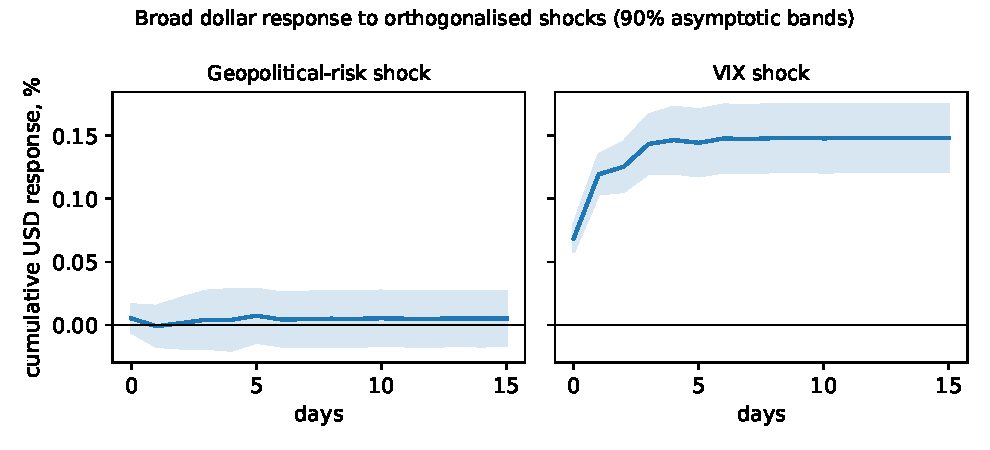
\includegraphics[width=\linewidth]{var_irf_gpr}
  \caption[Dollar impulse responses to risk and sentiment shocks]{Cumulative response of
  the broad dollar index to orthogonalised shocks, with $90\%$ asymptotic bands. The dollar
  does not respond to a geopolitical-risk shock (left) but appreciates significantly after a
  VIX shock (right).}
  \label{fig:var_irf}
\end{figure}


\section{Forecast Error Variance Decomposition}
\label{sec:svar_fevd}

The variance decomposition confirms the magnitudes. At a ten-day horizon, geopolitical-risk
shocks account for $0.1\%$ of the broad dollar's forecast-error variance, oil for $1.8\%$,
and the VIX for $7.9\%$; the remainder is the dollar's own innovations and the currency
baskets (Table~\ref{tab:var_fevd}). Whatever the geopolitical-risk index contributes to the
dollar, it does so not through a measurable daily linear channel but through the discrete,
high-salience events isolated in Chapter~\ref{ch:event_study}.

\begin{table}[htbp]
\centering
\begin{threeparttable}
\caption{Forecast error variance decomposition of the broad dollar (\%)}
\label{tab:var_fevd}
\small
\begin{tabular}{l rrrrrr}
\toprule
Horizon & $\Delta$GPR & Brent & $\Delta$VIX & Safe & Risky & USD own \\
\midrule
$h{=}1$  & $0.1$ & $1.1$ & $7.6$ & $49.9$ & $6.4$ & $34.9$ \\
$h{=}5$  & $0.1$ & $1.8$ & $7.9$ & $49.2$ & $6.4$ & $34.7$ \\
$h{=}10$ & $0.1$ & $1.8$ & $7.9$ & $49.2$ & $6.4$ & $34.7$ \\
\bottomrule
\end{tabular}
\begin{tablenotes}[flushleft]\footnotesize
\item \textit{Notes.} Share of the broad dollar's forecast-error variance attributable to
each orthogonalised shock, recursive ordering as in Section~\ref{sec:svar_diagnostics}.
\end{tablenotes}
\end{threeparttable}
\end{table}


\section{Interpretation and Caveats}
\label{sec:svar_subsample}

The VAR and the event study are two readings of the same object that agree once the
distinction between a \emph{level} and an \emph{event} is taken seriously. Geopolitical risk
moves the dollar when it arrives as a discrete, interpretable shock---an invasion, a tariff
announcement, a strait closure---whose direction the market can price; the running GPR
index, which also rises on diffuse, ambiguous news, carries no such daily signal and so
predicts nothing. Risk sentiment (the VIX) is the channel through which acute episodes reach
the dollar, which is why the safe-haven reflex shows up in the VIX impulse response.

Three caveats bound these results. First, identification rests on the recursive ordering;
plausible reorderings are examined in Appendix~\ref{ch:appendix_a} and leave the
qualitative picture unchanged. Second, a formal split into a tariff subsample and an Iran
subsample is not pursued: each window is too short for a stable six-variable VAR, and the
event study already provides the cleaner episode-by-episode identification. Third, the daily
GPR index is itself a noisy text-based measure, which biases its estimated daily effect
toward zero---a reason to read the null as ``no measurable linear daily channel'' rather
than ``no role for geopolitics,'' a role the event study documents directly.

% ---------- 08_discussion ----------

\chapter{Discussion}
\label{ch:discussion}

This chapter draws the event-study and VAR results together, relates them to the literature,
and sets out their implications and limits.

\section{The Dollar's Safe Haven Is Conditional on Shock Type}
\label{sec:disc_hierarchy}

The central finding is that the dollar's safe-haven response is conditioned by the
\emph{type} of shock, not merely by who causes it. The dollar appreciated around both
military/oil-supply shocks---the external Ukraine invasion and the U.S.-originated Hormuz
crisis---and the formal difference test cannot distinguish the two responses, even though
the United States authored one and merely witnessed the other. Yet it depreciated around the
one purely economic-policy shock it created, the Liberation Day tariffs. Origin alone does
not explain the pattern; the nature of the shock does. This refines the ``dollar-erosion''
reading \parencite{corsetti2025,kamin2025}: the safe-haven function is not weakening in
general but is specifically suspended when the United States is itself the source of an
economic-policy shock, while it survives intact---reversion notwithstanding---for the
security shocks that the safe-haven tradition has always emphasised
\parencite{ranaldo2010,habib2012}.

The structural VAR sharpens rather than contradicts this. Over the full sample, the running
geopolitical-risk index does not Granger-cause the dollar and explains almost none of its
variance, while risk sentiment (the VIX) does. The reconciliation is that the dollar
responds to geopolitics when it arrives as a discrete, interpretable event whose direction
markets can price---an invasion, a tariff list, a strait closure---and not to the diffuse,
continuously measured ``ambient'' risk that the index also captures. The safe-haven reflex
is event-driven, and it reaches the currency through the risk-sentiment channel.

\section{Gold and the Oil Channel}
\label{sec:disc_oil}

Gold does not behave as the universal safe haven that a first reading of
\textcite{baur2010} would predict. Instead it tracks the inverse of the dollar across the
U.S.-originated shocks---rising when the tariff shock weakened the dollar, falling when the
Hormuz shock strengthened it---and bids alongside the dollar only for the external Ukraine
shock. Gold is thus better described as a hedge \emph{against} the dollar than as a
substitute for it, which reinforces, rather than competes with, the chapter's main message:
the dollar's own conditional move is the organising variable, and gold prices it from the
other side.

The oil channel operates as the commodity-currency literature predicts, but only for the
supply shock. During the Hormuz crisis, oil-importer currencies underperformed
oil-exporters as crude surged, consistent with \textcite{chen2003} and \textcite{kilian2009};
during the demand-driven tariff decline the sorting was muted. The yen illustrates the
resulting tension: a classical safe haven that is also a large oil importer, it is pulled in
opposite directions during an oil-supply shock, which is part of why the basket responses
around Hormuz are smaller and noisier than the dollar-index response.

\section{Policy Implications}
\label{sec:disc_policy}

Three implications follow. For reserve managers and central banks, the dollar's safe-haven
status cannot be treated as unconditional: hedging programmes calibrated on the assumption
that the dollar always rallies in risk-off episodes will misfire precisely when the shock
originates in U.S.\ economic policy. For portfolio managers, diversification should be
thought of across \emph{shock types}, not only across assets---gold and competing-haven
currencies, not the dollar, carried the flight to quality in the tariff episode. For the
broader debate on the dollar's reserve role \parencite{obstfeld2023,jiang2026}, the evidence
is a caution against over-reading any single episode: the 2025 tariff shock did dent the
dollar, but the 2026 security shock showed the haven bid still firmly in place.

\section{Limitations}
\label{sec:disc_limitations}

Several caveats bound the results. The two most recent events---the May~2026 U.S.\ strikes
and the June~2026 ceasefire---have too few post-event trading days for the longer windows,
so they are reported only at short horizons. The structural VAR rests on a recursive
ordering and on a text-based daily risk index that is noisy, biasing its estimated daily
effect toward zero. Gold's exceptional 2025--26 trend makes its constant-mean CARs
sensitive in level, so they are read for sign rather than magnitude. As a single-country
event study around a small number of recent, partly overlapping episodes, the design trades
breadth for the clean U.S.-versus-external contrast; and without forward/basis data beyond
the one-month tenor, covered-interest-parity deviations are left for future work.

% ---------- 09_conclusion ----------

\chapter{Conclusion}
\label{ch:conclusion}

This thesis asked whether the U.S.\ dollar's safe-haven response depends on the type of
shock that triggers a crisis, even when the United States is implicated in the shock itself.
Two recent episodes provided an unusually clean test: the 2025 Liberation Day tariffs, a
purely U.S.\ economic-policy shock, and the 2026 Iran/Hormuz crisis, a geopolitical
oil-supply shock, with the 2022 Russian invasion of Ukraine as an external control.

The evidence gives a clear answer. The two shock types produced a mirror image. The dollar
depreciated around the tariff shock---roughly four percent on the broad index within twenty
trading days---while it appreciated around the Hormuz crisis and around Ukraine, and a formal
difference test confirms the tariff response is significantly distinct from both security
episodes, which are themselves statistically indistinguishable from one another. The dollar's
haven status is therefore conditional on the \emph{nature} of the shock, not on its origin:
it survives a U.S.-originated security shock but inverts for a U.S.-originated economic-policy
shock. The structural VAR adds that this is an event-driven phenomenon---the continuous
geopolitical-risk index does not move the dollar on an average day; risk sentiment is the
channel through which acute episodes reach it. Two further results round out the picture:
gold acts as a hedge against the dollar rather than as a universal safe haven, and the oil
channel sorts currencies only for the supply-driven shock.

The thesis contributes the first systematic side-by-side comparison of the Liberation Day and
Iran/Hormuz episodes for currency markets, carries a gold and oil benchmark through the same
design to connect the safe-haven and commodity-currency literatures, and extends standard
cross-sectional currency tools to mid-2026 on a consistent WMR dataset.

Several extensions suggest themselves. As the geopolitical situation continues to evolve, the
sample can be extended so that the most recent episodes acquire full post-event windows.
Richer forward and basis data would allow covered-interest-parity deviations to be brought
into the analysis, and intraday data would tighten the identification around the announcement
windows. A dynamic conditional-correlation (DCC-GARCH) model of the dollar--VIX relationship
would test the safe-haven-breakdown hypothesis directly and is the natural next layer.
Finally, a formal model of shock-dependent safe-haven demand---in which the currency of the
shock's originator loses its haven premium for policy shocks but not for security
shocks---would give the empirical pattern documented here a theoretical foundation.
\backmatter
\printbibliography[heading=head]

\chapter{Appendix A: Additional Tables and Notes}
\label{ch:appendix_a}

\section{Currency Universe and Classification}
\label{sec:app_classification}

Table~\ref{tab:app_ccy} lists the 32 currencies in the panel with their carry-sorted bucket
(low/middle/high forward-discount tercile, pegged and managed currencies excluded from the
sort) and their oil-trade role. The named safe-haven robustness baskets used in
Chapter~\ref{ch:event_study} are the yen, Swiss franc and euro (safe) against the Turkish
lira, Brazilian real, South African rand, Mexican peso, Colombian peso and Indonesian rupiah
(risky).

\begin{table}[htbp]
\centering
\begin{threeparttable}
\caption{Currency classification}
\label{tab:app_ccy}
\small
\begin{tabular}{ll l l}
\toprule
Code & Currency & Carry bucket & Oil role \\
\midrule
AUD & Australian dollar   & middle            & --- \\
BRL & Brazilian real      & high (risky)      & exporter \\
CAD & Canadian dollar     & middle            & exporter \\
CHF & Swiss franc         & low (safe)        & --- \\
CLP & Chilean peso        & no 1M forward     & --- \\
CNY & Chinese yuan        & pegged/managed    & --- \\
COP & Colombian peso      & no 1M forward     & exporter \\
CZK & Czech koruna        & middle            & --- \\
DKK & Danish krone        & pegged (EUR)      & --- \\
EUR & Euro                & low (safe)        & --- \\
GBP & Pound sterling      & middle            & --- \\
HKD & Hong Kong dollar    & pegged (USD)      & --- \\
HUF & Hungarian forint    & high (risky)      & --- \\
IDR & Indonesian rupiah   & high (risky)      & --- \\
ILS & Israeli shekel      & low (safe)        & --- \\
INR & Indian rupee        & high (risky)      & importer \\
JPY & Japanese yen        & low (safe)        & importer \\
KRW & South Korean won    & middle            & importer \\
KWD & Kuwaiti dinar       & pegged            & exporter \\
MXN & Mexican peso        & high (risky)      & exporter \\
MYR & Malaysian ringgit   & middle            & --- \\
NOK & Norwegian krone     & middle            & exporter \\
NZD & New Zealand dollar  & middle            & --- \\
PEN & Peruvian sol        & no 1M forward     & --- \\
PLN & Polish zloty        & high (risky)      & --- \\
SAR & Saudi riyal         & pegged            & exporter \\
SEK & Swedish krona       & low (safe)        & --- \\
SGD & Singapore dollar    & low (safe)        & --- \\
THB & Thai baht           & low (safe)        & importer \\
TRY & Turkish lira        & high (risky)      & importer \\
TWD & Taiwan dollar       & low (safe)        & importer \\
ZAR & South African rand  & high (risky)      & --- \\
\bottomrule
\end{tabular}
\begin{tablenotes}[flushleft]\footnotesize
\item \textit{Notes.} Carry buckets are terciles of the average one-month forward discount
(Section~\ref{sec:data_portfolios}); pegged/managed currencies and the three currencies
without a clean one-month forward (CLP, COP, PEN) are excluded from the carry sort. Oil role
follows the net oil-trade classification.
\end{tablenotes}
\end{threeparttable}
\end{table}

\section{Robustness}
\label{sec:app_robustness}

\paragraph{Market model.} Alongside the constant-mean specification, the event study computes
market-model abnormal returns for the individual currencies, using the equal-weighted dollar
factor as the market return (Code/\texttt{03\_event\_study.py}, method \texttt{market\_model}).
These are reported in the replication output; the safe-haven ordering across currencies is
unchanged relative to the constant-mean results in Chapter~\ref{ch:event_study}.

\paragraph{VAR identification.} The structural VAR places geopolitical risk \emph{first} in
the recursive ordering, so it is permitted to affect every other variable
contemporaneously. That geopolitical-risk innovations nonetheless neither Granger-cause the
dollar nor contribute materially to its forecast-error variance is therefore not an artefact
of a restrictive ordering---the ordering gives the index its best chance to matter. The
dollar's significant response to a VIX shock and its non-response to a geopolitical-risk
shock are robust to plausible reorderings of the three driver blocks.

\section{Data and Code Availability}
\label{sec:app_data}

All data are daily, 1~January 2019 to 30~June 2026. The macro-financial block (dollar
indices, Treasury and TIPS yields, breakeven inflation, the VIX, Brent and WTI crude, Henry
Hub gas, and the S\&P~500) is from FRED. The 32-currency spot and one-month forward panel,
gold, the Euro Stoxx~50, and the TTF gas contract are exported from LSEG at the WM/Reuters
fixing. The Geopolitical Risk index is from Caldara and Iacoviello, and the Economic and
Trade Policy Uncertainty indices from \textit{policyuncertainty.com}. The analysis pipeline
(\texttt{consolidate\_lseg.py} $\to$ \texttt{get\_data.py} $\to$ \texttt{build\_fx\_factors.py}
$\to$ \texttt{02\_build\_returns.py} $\to$ \texttt{03}/\texttt{04}/\texttt{05}/\texttt{06})
reproduces every table and figure in the thesis from these sources.


\chapter{Affidavit}
\thispagestyle{empty}

\begin{german}
	Ich versichere, dass ich die vorliegende Arbeit ohne Hilfe Dritter und ohne Benutzung anderer
	als der angegebenen Quellen und Hilfsmittel angefertigt und die den benutzten Quellen
	wörtlich oder inhaltlich entnommenen Stellen als solche kenntlich gemacht habe. Diese Arbeit
	hat in gleicher oder ähnlicher Form noch keiner Prüfungsbehörde vorgelegen.
	
	Ich bin damit einverstanden, dass meine Arbeit zum Zwecke eines Plagiatsabgleichs in
	elektronischer Form anonymisiert versendet und gespeichert werden kann.
\end{german}

\vspace{\baselineskip}


\noindent I affirm that this Bachelor thesis was written by myself without any unauthorised third-party support.
All used references and resources are clearly indicated. All quotes and citations are properly referenced.
This thesis was never presented in the past in the same or similar form to any examination board.

I agree that my thesis may be subject to electronic plagiarism check. 
For this purpose an anonymous copy may be distributed and uploaded to servers within and outside the University of Mannheim.

\vspace{4\baselineskip}
\begin{center}
\parbox{.8\textwidth}{Mannheim, \today \hfill Signature}
\end{center}

\endinput
\end{document}